% =============================================================================
% Praxisprojektarbeit (PPA)
% Decubitus Detection for the NaMeKI Project:
% Data Foundation and Model Selection
%
% Author:  Ashkan Sadri Ghamshi (769529)
% HAWK -- Hochschule fur angewandte Wissenschaft und Kunst
% Fakultat Ingenieurwissenschaften und Gesundheit
%
% Compiled with tectonic (XeLaTeX-based)
% =============================================================================

\documentclass[a4paper,12pt,twoside]{report}

% ---------------------------------------------------------------------------
% Geometry
% ---------------------------------------------------------------------------
\usepackage[
  left=3cm,
  right=2.5cm,
  top=2.5cm,
  bottom=2.5cm,
  bindingoffset=0.5cm
]{geometry}

% ---------------------------------------------------------------------------
% Encoding and fonts
% ---------------------------------------------------------------------------
\usepackage[T1]{fontenc}
\usepackage[utf8]{inputenc}
\usepackage{lmodern}
\usepackage{microtype}

% ---------------------------------------------------------------------------
% Language
% ---------------------------------------------------------------------------
\usepackage[english]{babel}

% ---------------------------------------------------------------------------
% Mathematics
% ---------------------------------------------------------------------------
\usepackage{amsmath}
\usepackage{amssymb}

% ---------------------------------------------------------------------------
% Graphics and colour
% ---------------------------------------------------------------------------
\usepackage{graphicx}
\usepackage{xcolor}
\usepackage{subcaption}
\usepackage{enumitem}

% ---------------------------------------------------------------------------
% Tables
% ---------------------------------------------------------------------------
\usepackage{booktabs}
\usepackage{tabularx}
\usepackage{array}
\usepackage{multirow}
\usepackage{longtable}

% ---------------------------------------------------------------------------
% Code listings
% ---------------------------------------------------------------------------
\usepackage{listings}
\lstset{
  language=Python,
  basicstyle=\ttfamily\small,
  keywordstyle=\color{blue}\bfseries,
  commentstyle=\color{gray}\itshape,
  stringstyle=\color{red!70!black},
  numbers=left,
  numberstyle=\tiny\color{gray},
  numbersep=8pt,
  frame=single,
  breaklines=true,
  breakatwhitespace=false,
  showstringspaces=false,
  tabsize=4,
  captionpos=b,
  aboveskip=10pt,
  belowskip=10pt
}

% ---------------------------------------------------------------------------
% Hyperlinks
% ---------------------------------------------------------------------------
\usepackage{hyperref}
\hypersetup{
  colorlinks=true,
  linkcolor=black,
  citecolor=blue!60!black,
  urlcolor=blue!70!black,
  pdfauthor={Ashkan Sadri Ghamshi},
  pdftitle={Decubitus Detection -- Data Foundation and Model Selection},
  pdfsubject={Praxisprojektarbeit, HAWK University},
}

% ---------------------------------------------------------------------------
% Bibliography (natbib, numeric)
% ---------------------------------------------------------------------------
\usepackage[numbers,square,sort&compress]{natbib}

% ---------------------------------------------------------------------------
% Chapter-relative numbering (Ibenthal guideline)
% ---------------------------------------------------------------------------
\usepackage{chngcntr}
\counterwithin{equation}{chapter}
\counterwithin{figure}{chapter}
\counterwithin{table}{chapter}

% ---------------------------------------------------------------------------
% Headers and footers
% ---------------------------------------------------------------------------
\usepackage{fancyhdr}
\pagestyle{fancy}
\fancyhf{}
\fancyhead[LE]{\leftmark}
\fancyhead[RO]{\rightmark}
\fancyfoot[C]{\thepage}
\renewcommand{\headrulewidth}{0.4pt}
\renewcommand{\footrulewidth}{0pt}

% ---------------------------------------------------------------------------
% Paragraph formatting
% ---------------------------------------------------------------------------
\setlength{\parindent}{0pt}
\setlength{\parskip}{6pt plus 2pt minus 1pt}

% ---------------------------------------------------------------------------
% Glossary (manual, lightweight -- no extra package needed)
% ---------------------------------------------------------------------------
% We define a simple glossary environment using description lists.

% ---------------------------------------------------------------------------
% Depth of numbering
% ---------------------------------------------------------------------------
\setcounter{secnumdepth}{3}
\setcounter{tocdepth}{3}

% ============================================================================
%  DOCUMENT START
% ============================================================================
\begin{document}

% ============================================================================
%  TITLE PAGE
% ============================================================================
\begin{titlepage}
  \centering
  \vspace*{1.5cm}

  {\Large\bfseries HAWK}\\[4pt]
  {\normalsize Hochschule f{\"u}r angewandte Wissenschaft und Kunst\\
  Hildesheim/Holzminden/G{\"o}ttingen}\\[6pt]
  {\normalsize Fakult{\"a}t Ingenieurwissenschaften und Gesundheit}

  \vspace{2.5cm}

  {\LARGE\bfseries Praxisprojektarbeit}\\[12pt]
  {\Large\bfseries Decubitus Detection for the NaMeKI Project:\\
  Data Foundation and Model Selection}

  \vspace{2.5cm}

  \begin{tabular}{ll}
    \textbf{Author:}          & Ashkan Sadri Ghamshi \\
    \textbf{Matriculation No.:} & 769529 \\[6pt]
    \textbf{Supervisor:}      & Prof.\ Dr.\ Claire Chalopin \\
                               & Gesundheitscampus G{\"o}ttingen \\[6pt]
    \textbf{Date:}            & April 1, 2026
  \end{tabular}

  \vfill
\end{titlepage}

% ============================================================================
%  SELBSTANDIGKEITSERKLARUNG
% ============================================================================
\clearpage
\thispagestyle{empty}
\vspace*{3cm}
\begin{center}
  {\Large\bfseries Selbst{\"a}ndigkeitserkl{\"a}rung}
\end{center}

\vspace{1.5cm}

Hiermit erkl{\"a}re ich, dass ich die vorliegende Arbeit selbst{\"a}ndig und ohne
unzul{\"a}ssige Hilfe Dritter angefertigt habe. Alle Stellen, die inhaltlich oder
w{\"o}rtlich aus Ver{\"o}ffentlichungen oder anderen Quellen entnommen sind, habe
ich als solche kenntlich gemacht. Die Arbeit wurde bisher weder im Inland noch
im Ausland in gleicher oder {\"a}hnlicher Form einer Pr{\"u}fungsbeh{\"o}rde vorgelegt.

\vspace{3cm}

\begin{tabular}{p{6cm}p{6cm}}
  \hrulefill & \hrulefill \\
  Ort, Datum & Unterschrift
\end{tabular}

% ============================================================================
%  ABSTRACT
% ============================================================================
\clearpage
\thispagestyle{empty}
\vspace*{2cm}
\begin{center}
  {\Large\bfseries Abstract}
\end{center}
\vspace{1cm}

Pressure ulcers remain a significant clinical challenge in nursing care, affecting
patient quality of life and placing substantial financial burden on healthcare
systems. This Praxisprojektarbeit establishes the data foundation for an
automated pressure ulcer detection system within the NaMeKI research project at
HAWK University. A total of 20,080 raw wound images were collected from eleven
publicly available datasets across three platforms, consolidated into 7,850
unique images through perceptual-hash-based deduplication, and expanded to
53,340 annotated samples via a controlled augmentation pipeline. A
literature-based comparison of four deep learning architectures---YOLOv8,
DenseNet-121, EfficientNet-B0, and Faster R-CNN---using a weighted scoring
matrix identifies YOLOv8s as the most suitable model, given its combined
detection and localisation capability, published mean average precision of
90.8\,\% on comparable data, and real-time inference performance.

% ============================================================================
%  TABLE OF CONTENTS
% ============================================================================
\clearpage
\tableofcontents

% ============================================================================
%  LIST OF FIGURES / TABLES
% ============================================================================
\clearpage
\listoffigures
\clearpage
\listoftables

% ============================================================================
%  GLOSSARY
% ============================================================================
\clearpage
\chapter*{Glossary}
\addcontentsline{toc}{chapter}{Glossary}

\begin{description}[leftmargin=4cm, style=nextline]

\item[AI] Artificial Intelligence. A branch of computer science concerned with
  building systems that can perform tasks normally requiring human cognition.

\item[Bounding Box] A rectangular region in an image that encloses an object of
  interest, typically represented by centre coordinates, width, and height.

\item[CLAHE] Contrast-Limited Adaptive Histogram Equalisation. An image
  processing technique that improves local contrast without amplifying noise.

\item[CNN] Convolutional Neural Network. A class of deep neural networks
  primarily used for visual pattern recognition.

\item[COCO] Common Objects in Context. A large-scale benchmark dataset and
  evaluation protocol for object detection and segmentation \citep{lin2014coco}.

\item[CSPDarknet] Cross-Stage Partial Darknet. The backbone architecture used
  in YOLOv8 for feature extraction.

\item[Decubitus] A pressure ulcer or pressure injury caused by sustained
  mechanical loading on the skin and underlying tissue.

\item[DenseNet] Densely Connected Convolutional Network \citep{huang2017densely}.
  A CNN architecture in which each layer receives input from all preceding layers.

\item[DTI] Deep Tissue Injury. A pressure-related injury characterised by
  localised discolouration of intact skin.

\item[EfficientNet] A family of CNN architectures that use compound scaling to
  balance network depth, width, and resolution \citep{tan2019efficientnet}.

\item[EPUAP] European Pressure Ulcer Advisory Panel. An organisation that
  co-publishes international pressure injury classification guidelines.

\item[FPS] Frames Per Second. A measure of inference throughput.

\item[IoU] Intersection over Union. A metric quantifying overlap between a
  predicted bounding box and a ground truth bounding box.

\item[mAP] Mean Average Precision. The primary evaluation metric for object
  detection models, computed across all classes and IoU thresholds.

\item[MPS] Metal Performance Shaders. Apple's GPU computation framework used as
  a PyTorch backend on Apple Silicon hardware.

\item[NaMeKI] \textit{Nachhaltige Mensch-KI-Interaktion.} The HAWK research
  project within which this work is situated.

\item[NPUAP] National Pressure Injury Advisory Panel. The US body that defines
  pressure ulcer staging categories \citep{npuap2019staging}.

\item[ONNX] Open Neural Network Exchange. An open format for representing
  trained deep learning models, enabling cross-framework deployment.

\item[PANet] Path Aggregation Network. A feature pyramid architecture used in
  the neck of YOLOv8 for multi-scale feature fusion.

\item[Perceptual Hash] A fingerprinting technique that produces similar hash
  values for visually similar images, enabling near-duplicate detection.

\item[PPA] Praxisprojektarbeit. A practical project report required as part of
  the degree programme at HAWK University.

\item[PU] Pressure Ulcer. Synonymous with pressure injury or decubitus.

\item[ROI] Region of Interest. A subregion of an image relevant to analysis.

\item[YOLO] You Only Look Once \citep{redmon2016yolo}. A family of single-stage
  object detection architectures known for real-time inference speed.

\item[YOLOv8] The eighth major iteration of the YOLO architecture, developed by
  Ultralytics \citep{jocher2023yolov8}.

\end{description}

% ============================================================================
%  MAIN MATTER
% ============================================================================
\clearpage
\pagenumbering{arabic}

% ============================================================================
%  CHAPTER 1 -- INTRODUCTION
% ============================================================================
\chapter{Introduction}
\label{ch:introduction}

Pressure ulcers, also referred to as pressure injuries or decubitus wounds,
constitute one of the most prevalent adverse events in healthcare facilities
worldwide. These lesions arise from sustained mechanical loading on skin and
underlying tissues, typically over bony prominences, and disproportionately
affect patients with limited mobility such as the elderly, individuals with
spinal cord injuries, and intensive care patients \citep{npuap2019staging}. Early
detection and accurate staging of pressure ulcers are essential for initiating
timely treatment and preventing progression to deeper tissue damage. Despite
decades of clinical research and prevention protocols, incidence rates remain
high, with estimates indicating that between 5\,\% and 15\,\% of hospitalised
patients develop at least one pressure ulcer during their stay
\citep{busupalli2023healthcare}.

The economic impact of pressure ulcers on healthcare systems is substantial.
Treatment costs per patient can range from several thousand to tens of thousands
of euros, depending on the severity of the wound and associated complications
such as infection and prolonged hospitalisation \citep{dealey2005skin}. Beyond
the financial dimension, pressure ulcers significantly reduce patient quality of
life, cause pain, and increase morbidity and mortality. These factors collectively
underscore the clinical imperative for improved detection methodologies.

\section{Project Context}
\label{sec:project-context}

This Praxisprojektarbeit is conducted within the NaMeKI
(\textit{Nachhaltige Mensch-KI-Interaktion}) research project at HAWK
University, Gesundheitscampus G{\"o}ttingen. The NaMeKI project investigates
sustainable human--AI interaction paradigms in healthcare settings, with pressure
ulcer detection serving as a primary application domain. The overarching goal is
to develop a camera-based monitoring system that can automatically detect and
classify pressure ulcers on patient skin, thereby assisting nursing staff in
clinical decision-making.

Within this broader project context, the present work focuses exclusively on two
foundational tasks: (1)~the systematic collection, curation, and augmentation of
a high-quality training dataset, and (2)~a literature-based comparison and
justified selection of a suitable deep learning architecture for subsequent model
training. The actual training, fine-tuning, and integration of the selected model
into the NaMeKI system are deferred to the subsequent bachelor thesis.

\section{Motivation}
\label{sec:motivation}

Manual assessment of pressure ulcers by nursing personnel is inherently
subjective. Studies have shown that inter-rater reliability for pressure ulcer
staging varies considerably, particularly for intermediate stages where visual
differentiation between categories can be challenging. Automated detection
systems based on deep learning have the potential to reduce this variability by
providing consistent, reproducible classifications.

However, the development of such systems depends critically on the availability
of representative training data. Medical image datasets for pressure ulcers are
scarce compared to general-purpose computer vision benchmarks. Existing datasets
are fragmented across multiple platforms, vary in annotation format and quality,
and frequently contain duplicate images. Furthermore, class distributions in
clinical datasets tend to be imbalanced, with certain wound stages
overrepresented. Addressing these data challenges is a prerequisite for training
a model that generalises reliably across different wound presentations.

Equally important is the selection of an appropriate model architecture. The
choice between classification-only models and detection models, between
single-stage and two-stage detectors, and among different network capacities has
direct implications for the system's accuracy, inference speed, and deployability
within the NaMeKI platform. A systematic, criteria-based comparison is therefore
necessary to justify the architectural decision.

\section{Objectives}
\label{sec:objectives}

This Praxisprojektarbeit pursues the following objectives:

\begin{enumerate}
  \item \textbf{Dataset Collection:} Identify and download publicly available
    pressure ulcer image datasets from Roboflow, GitHub, and Kaggle, targeting a
    minimum of 10,000 raw images.

  \item \textbf{Data Curation:} Unify annotation formats to YOLO bounding box
    format, remove duplicate and low-quality images through perceptual hashing,
    and establish a consistent four-class labelling scheme aligned with
    NPUAP/EPUAP staging categories.

  \item \textbf{Data Augmentation:} Design and implement an augmentation pipeline
    using the Albumentations library that preserves bounding box annotations and
    expands the training set by a configurable factor.

  \item \textbf{Architecture Comparison:} Conduct a literature-based comparison
    of YOLOv8, DenseNet-121, EfficientNet-B0, and Faster~R-CNN using a weighted
    scoring matrix that considers detection capability, published performance on
    pressure ulcer data, inference speed, implementation complexity, and
    deployment readiness.

  \item \textbf{Model Recommendation:} Provide a justified recommendation for
    the model architecture and variant to be used in the subsequent bachelor
    thesis.

  \item \textbf{Documentation:} Document the entire data pipeline and
    decision-making process in a reproducible manner.
\end{enumerate}

\section{Scope and Delimitation}
\label{sec:scope}

The scope of this work is limited to data preparation and model selection. The
following activities are explicitly excluded and reserved for the subsequent
bachelor thesis:

\begin{itemize}
  \item Training, fine-tuning, or evaluating any deep learning model on the
    prepared dataset.
  \item Developing a prototype application or integrating detection capabilities
    into the NaMeKI system.
  \item Collecting proprietary clinical data from healthcare facilities.
  \item Addressing ethical approval for patient data, as only publicly available
    datasets are used.
\end{itemize}

The clinical focus is on pressure ulcer stages~I through~IV according to the
NPUAP/EPUAP classification system. Unstageable wounds and deep tissue injuries
are excluded from the current four-class scheme but can be incorporated in future
extensions of the dataset.

\section{Chapter Overview}
\label{sec:chapter-overview}

The remainder of this report is organised as follows.
Chapter~\ref{ch:system-overview} provides a high-level system overview of the
data pipeline and its interfaces. Chapter~\ref{ch:state-of-art} reviews the
state of the art in pressure ulcer detection using deep learning.
Chapter~\ref{ch:requirements} analyses the functional and non-functional
requirements for the dataset and model selection.
Chapter~\ref{ch:concept} presents the concept development, including the problem
analysis and solution approach. Chapter~\ref{ch:implementation} details the
implementation of the data collection, cleaning, deduplication, and augmentation
pipeline. Chapter~\ref{ch:testing} describes the testing and validation strategy
applied to the prepared dataset. Chapter~\ref{ch:benchmarking} presents the
architecture comparison and scoring results.
Chapter~\ref{ch:conclusion} summarises the contributions, discusses challenges
encountered, and outlines open points for the bachelor thesis.

% ============================================================================
%  CHAPTER 2 -- SYSTEM OVERVIEW
% ============================================================================
\chapter{System Overview}
\label{ch:system-overview}

This chapter provides a high-level view of the data preparation system developed
in this Praxisprojektarbeit. The system transforms heterogeneous raw image data
from multiple public sources into a unified, augmented, and validated dataset
suitable for training an object detection model. Understanding the overall
architecture and the interfaces between components is essential before examining
individual pipeline stages in subsequent chapters.

\section{Block Diagram}
\label{sec:block-diagram}

The data pipeline consists of five principal stages arranged in a sequential
processing chain. Figure~\ref{fig:pipeline-block} illustrates the logical flow
from raw data acquisition to the final validated dataset.

\begin{figure}[htbp]
  \centering
  \fbox{\parbox{0.9\textwidth}{%
    \centering
    \vspace{8pt}
    \textbf{Stage 1: Data Collection}\\
    (Roboflow API, GitHub, Kaggle)\\[4pt]
    $\downarrow$ \quad 20{,}080 raw images \\[6pt]
    \textbf{Stage 2: Format Unification}\\
    (Mask-to-BBox conversion, class remapping)\\[4pt]
    $\downarrow$ \quad Unified YOLO format \\[6pt]
    \textbf{Stage 3: Deduplication \& Quality Control}\\
    (Perceptual hashing, resolution filtering)\\[4pt]
    $\downarrow$ \quad 7{,}850 unique images \\[6pt]
    \textbf{Stage 4: Train/Val/Test Split}\\
    (70\,\% / 20\,\% / 10\,\%)\\[4pt]
    $\downarrow$ \quad Stratified partitions \\[6pt]
    \textbf{Stage 5: Augmentation}\\
    (Albumentations, 10$\times$ expansion)\\[4pt]
    $\downarrow$ \quad 53{,}340 augmented images \\[2pt]
    \vspace{4pt}
  }}
  \caption{Block diagram of the data preparation pipeline. Each stage receives
    input from the preceding stage and produces output in a standardised format.
    Numeric values indicate the dataset size at each transition point.}
  \label{fig:pipeline-block}
\end{figure}

\section{Interface Description}
\label{sec:interfaces}

The interfaces between pipeline stages are defined by the file system structure
and the YOLO annotation format. All inter-stage data exchange follows a
consistent directory layout:

\begin{itemize}
  \item \texttt{images/<split>/} contains the image files (JPEG or PNG) for each
    data split (train, val, test).
  \item \texttt{labels/<split>/} contains the corresponding YOLO-format
    annotation files, where each \texttt{.txt} file shares the filename stem of
    its associated image.
  \item \texttt{dataset.yaml} specifies the dataset root path, split
    directories, number of classes, and class name mapping.
\end{itemize}

Each annotation file contains one line per bounding box in the format:

\begin{center}
  \texttt{<class\_id> <centre\_x> <centre\_y> <width> <height>}
\end{center}

where all spatial coordinates are normalised to the range $[0, 1]$ relative to
the image dimensions. This format is directly compatible with the Ultralytics
YOLOv8 training framework \citep{jocher2023yolov8}.

\section{External Interfaces}
\label{sec:external-interfaces}

The system interfaces with three external data sources:

\begin{enumerate}
  \item \textbf{Roboflow Universe:} Seven datasets are downloaded
    programmatically via the Roboflow Python API using an authenticated API key.
    Datasets are requested in YOLOv8 format, eliminating the need for annotation
    conversion for these sources.

  \item \textbf{GitHub Repositories:} Two datasets are cloned from public
    repositories. These datasets use segmentation masks rather than bounding box
    annotations, requiring a mask-to-bounding-box conversion step.

  \item \textbf{Kaggle:} Two datasets are downloaded via the Kaggle API. These
    sources provide images with varying annotation formats that are normalised
    during the unification stage.
\end{enumerate}

The output interface of the pipeline is the \texttt{dataset.yaml} configuration
file, which serves as the single entry point for the YOLOv8 training framework
in the subsequent bachelor thesis phase.

This chapter has established the high-level structure and interfaces of the data
preparation system. The following chapter examines the scientific and technical
foundations upon which this system is built, reviewing existing approaches to
pressure ulcer detection in the literature.

% ============================================================================
%  CHAPTER 3 -- STATE OF THE ART
% ============================================================================
\chapter{State of the Art}
\label{ch:state-of-art}

A thorough understanding of existing work in pressure ulcer detection and deep
learning for medical image analysis is necessary to position this project within
the current research landscape and to identify the gaps that the present work
addresses. This chapter reviews the clinical background of pressure ulcer
staging, surveys deep learning approaches applied to wound detection, examines
the evaluation metrics used in the field, and identifies limitations in existing
solutions.

\section{Clinical Background}
\label{sec:clinical-background}

Pressure ulcers are classified according to the depth of tissue damage using the
staging system defined by the NPUAP and EPUAP \citep{npuap2019staging}. This
classification system comprises four primary categories and two supplementary
categories:

\begin{description}
  \item[Stage~I:] Non-blanchable erythema of intact skin. The affected area
    presents persistent redness that does not blanch under finger pressure. No
    open wound is present, making this stage the most difficult to detect
    visually and the most susceptible to inter-rater variability.

  \item[Stage~II:] Partial-thickness skin loss presenting as a shallow open
    ulcer with a red or pink wound bed, without slough. This stage may also
    present as an intact or ruptured serum-filled blister. The visible wound
    boundary makes Stage~II more amenable to automated detection than Stage~I.

  \item[Stage~III:] Full-thickness skin loss in which subcutaneous fat may be
    visible, but bone, tendon, and muscle are not exposed. Slough may be present
    but does not obscure the depth of tissue loss.

  \item[Stage~IV:] Full-thickness tissue loss with exposed bone, tendon, or
    muscle. Slough or eschar may be present on parts of the wound bed. This
    represents the most severe category of pressure injury.
\end{description}

Additionally, the NPUAP defines unstageable wounds (depth unknown due to
coverage by slough or eschar) and deep tissue injuries (localised
discolouration of intact skin indicating damage to underlying tissue). These
supplementary categories are excluded from the current four-class scheme of this
project but may be incorporated in future dataset extensions.

\section{Deep Learning for Wound Detection}
\label{sec:dl-wound-detection}

The application of convolutional neural networks to pressure ulcer analysis has
followed two principal methodological directions: image classification and
object detection.

\subsection{Classification-Based Approaches}

Classification-based methods assign a wound stage label to an entire image or
to a pre-segmented region of interest. Ay et al.\ \citep{ay2022deep} applied
transfer learning with DenseNet-121 and EfficientNet-B0 to classify pressure
injury images from the PIID dataset (1,091 images) into four stages, achieving
classification accuracies of 83.6\,\% and 80.2\,\%, respectively. While these
results demonstrate the feasibility of automated staging, classification-only
models cannot localise wounds within an image. In clinical practice, knowing
\textit{where} a pressure ulcer is located on the patient's body is as important
as knowing its stage.

Zahia et al.\ \citep{zahia2020tissue} developed a custom CNN architecture for
tissue classification in pressure ulcer images, reporting an accuracy of
91.4\,\% on a dataset of 600 images. However, this approach operated on
pre-cropped tissue patches rather than whole images, which limits its
applicability to scenarios where manual region-of-interest selection has already
occurred.

\subsection{Detection-Based Approaches}

Object detection models simultaneously classify and localise objects within an
image by predicting bounding boxes and associated class labels. This paradigm
is more suitable for clinical deployment, where the system must identify the
location, extent, and stage of each wound in an image without prior manual
cropping.

Lau et al.\ \citep{lau2024yolov8} applied YOLOv8 to pressure ulcer detection
and staging on a dataset of 2,811 images, achieving a mean average precision at
50\,\% IoU threshold (mAP@50) of 90.8\,\%. This study demonstrated that
single-stage detectors can achieve competitive performance on medical wound
images while maintaining real-time inference speeds.

Faster~R-CNN \citep{ren2015faster}, a two-stage detector that first generates
region proposals and then classifies each proposal, has also been applied to
wound detection tasks. While two-stage detectors traditionally achieve higher
accuracy than single-stage approaches on general benchmarks, their inference
latency is substantially higher, and recent single-stage architectures such as
YOLOv8 have narrowed or eliminated this accuracy gap.

\section{Evaluation Metrics}
\label{sec:eval-metrics}

The evaluation of object detection models relies on metrics that account for
both classification accuracy and localisation precision. The primary metrics
used in the literature are:

\begin{description}
  \item[Precision:] The ratio of true positive detections to the total number
    of detections. A detection is considered a true positive if its IoU with a
    ground truth bounding box exceeds a defined threshold.

  \item[Recall:] The ratio of true positive detections to the total number of
    ground truth objects. High recall indicates that the model detects most of
    the wounds present in the image.

  \item[mAP@50:] Mean Average Precision computed at an IoU threshold of 0.50.
    This is the most commonly reported metric in pressure ulcer detection studies
    and serves as the primary comparison criterion in this work.

  \item[mAP@50:95:] Mean Average Precision averaged over IoU thresholds from
    0.50 to 0.95 in steps of 0.05. This stricter metric penalises imprecise
    bounding box localisation more heavily.

  \item[Classification Accuracy:] The proportion of correctly classified images.
    This metric is applicable only to classification models (e.g., DenseNet,
    EfficientNet) and does not assess localisation performance.
\end{description}

The use of different metrics across studies complicates direct comparison.
Classification models report accuracy, while detection models report mAP. This
discrepancy is addressed in the scoring matrix presented in
Chapter~\ref{ch:benchmarking}, where each model is evaluated on criteria that
are appropriate to its architectural category.

\section{Identified Gaps}
\label{sec:gaps}

The review of existing work reveals several gaps that this project addresses:

\begin{enumerate}
  \item \textbf{Dataset fragmentation:} Pressure ulcer datasets are distributed
    across multiple platforms (Roboflow, GitHub, Kaggle) without standardised
    annotation formats. No consolidated, multi-source dataset exists for
    four-class pressure ulcer detection.

  \item \textbf{Limited dataset sizes:} Most published studies operate on
    datasets of fewer than 3,000 images. The performance ceiling imposed by
    small training sets is a recognised limitation in the field.

  \item \textbf{Duplicate contamination:} Combining datasets from multiple
    sources without deduplication risks data leakage, where identical or
    near-identical images appear in both training and validation splits.

  \item \textbf{Inconsistent class definitions:} Different datasets use
    different labelling conventions (e.g., stage numbers, wound type names,
    varying granularity). A unified class mapping is required to train a single
    model across all sources.

  \item \textbf{Lack of systematic model comparison:} While individual studies
    report results for specific architectures, no systematic comparison of
    classification and detection models for pressure ulcer analysis has been
    published that accounts for deployment constraints such as inference speed
    and integration complexity.
\end{enumerate}

This chapter has established the scientific context for the present work. The
following chapter translates the identified gaps and project objectives into
concrete functional and non-functional requirements.

% ============================================================================
%  CHAPTER 4 -- REQUIREMENTS ANALYSIS
% ============================================================================
\chapter{Requirements Analysis}
\label{ch:requirements}

The requirements for this Praxisprojektarbeit derive from the NaMeKI project
objectives, the supervisor's specifications, and the gaps identified in the
state-of-the-art review. This chapter formalises these requirements and defines
use cases for the data pipeline. A clear requirements specification ensures that
the subsequent concept and implementation can be evaluated against defined
acceptance criteria.

\section{Functional Requirements}
\label{sec:func-req}

Table~\ref{tab:functional-req} lists the functional requirements for the data
preparation pipeline and model selection process.

\begin{table}[htbp]
  \centering
  \caption{Functional requirements for the data preparation pipeline.}
  \label{tab:functional-req}
  \begin{tabularx}{\textwidth}{lX}
    \toprule
    \textbf{ID} & \textbf{Requirement} \\
    \midrule
    FR-01 & The system shall download pressure ulcer image datasets from at least
            three public sources (Roboflow, GitHub, Kaggle). \\
    FR-02 & The system shall convert segmentation masks to YOLO bounding box
            format using contour extraction. \\
    FR-03 & The system shall map all source-specific class labels to a unified
            four-class scheme (Stage~1, Stage~2, Stage~3, Stage~4). \\
    FR-04 & The system shall detect and remove duplicate and near-duplicate
            images using perceptual hashing with a configurable similarity
            threshold. \\
    FR-05 & The system shall split the deduplicated dataset into training,
            validation, and test partitions with a 70\,\%/20\,\%/10\,\% ratio. \\
    FR-06 & The system shall augment the training partition using geometric,
            colour, and noise transformations while preserving bounding box
            annotations. \\
    FR-07 & The augmentation factor shall be configurable, with a default of
            $10\times$ expansion. \\
    FR-08 & The system shall produce a \texttt{dataset.yaml} configuration file
            compatible with the Ultralytics YOLOv8 framework. \\
    FR-09 & The model comparison shall evaluate at least four architectures using
            a weighted scoring matrix with documented criteria. \\
    FR-10 & The system shall generate statistical reports on class distribution,
            image dimensions, bounding box characteristics, and annotation
            density. \\
    \bottomrule
  \end{tabularx}
\end{table}

\section{Non-Functional Requirements}
\label{sec:nonfunc-req}

Table~\ref{tab:nonfunctional-req} specifies the non-functional requirements that
constrain the implementation.

\begin{table}[htbp]
  \centering
  \caption{Non-functional requirements.}
  \label{tab:nonfunctional-req}
  \begin{tabularx}{\textwidth}{lX}
    \toprule
    \textbf{ID} & \textbf{Requirement} \\
    \midrule
    NF-01 & All processing shall execute on a local workstation (Apple~M2~Ultra)
            without requiring cloud GPU resources. \\
    NF-02 & Image data shall not be committed to the Git repository; only scripts,
            configurations, and documentation shall be version-controlled. \\
    NF-03 & The pipeline shall be implemented in Python using standard scientific
            computing libraries (OpenCV, Albumentations, PIL, NumPy). \\
    NF-04 & Processing scripts shall include progress bars and status output to
            enable monitoring of long-running operations. \\
    NF-05 & The deduplication step shall complete within a reasonable time frame
            (under one hour for 20,000 images). \\
    NF-06 & All augmented images shall maintain a minimum resolution of
            $320 \times 320$ pixels. \\
    NF-07 & The dataset structure shall be extensible to support additional
            classes (unstageable, DTI) in future work. \\
    NF-08 & All scripts shall be executable via command-line arguments without
            hardcoded file paths. \\
    \bottomrule
  \end{tabularx}
\end{table}

\section{Use Cases}
\label{sec:use-cases}

Three primary use cases describe the interactions between the developer and the
data pipeline system.

\subsection{Use Case 1: Dataset Acquisition}

\textbf{Actor:} Developer.\\
\textbf{Precondition:} API keys for Roboflow and Kaggle are configured in
environment variables.\\
\textbf{Main Flow:} The developer executes the download scripts, which
programmatically retrieve datasets from each source and store them in the
\texttt{data/raw/} directory hierarchy.\\
\textbf{Postcondition:} Raw images and their associated annotations are stored
locally, organised by source.

\subsection{Use Case 2: Data Curation}

\textbf{Actor:} Developer.\\
\textbf{Precondition:} Raw datasets are available in \texttt{data/raw/}.\\
\textbf{Main Flow:} The developer sequentially executes the mask conversion,
class remapping, deduplication, and splitting scripts. Each script reads from
the previous stage's output directory and writes to the next.\\
\textbf{Postcondition:} A deduplicated, consistently labelled dataset is
partitioned into train, validation, and test splits in \texttt{data/unified/}.

\subsection{Use Case 3: Dataset Augmentation}

\textbf{Actor:} Developer.\\
\textbf{Precondition:} The unified dataset exists in \texttt{data/unified/} with
correctly formatted YOLO annotations.\\
\textbf{Main Flow:} The developer executes the augmentation script with a
specified expansion factor. The script applies stochastic transformations to each
training image and generates the configured number of augmented copies.\\
\textbf{Postcondition:} An augmented dataset is available in
\texttt{data/augmented/}, ready for training.

This chapter has defined the complete set of requirements governing the data
pipeline and model selection process. The following chapter translates these
requirements into a concrete concept and solution approach.

% ============================================================================
%  CHAPTER 5 -- CONCEPT DEVELOPMENT
% ============================================================================
\chapter{Concept Development}
\label{ch:concept}

With the requirements established, this chapter develops the conceptual
framework for the data pipeline and model selection methodology. The chapter
begins with a structured problem analysis, proceeds to the solution approach,
and concludes with the detailed design of the data pipeline and augmentation
strategy. The goal is to bridge the gap between the abstract requirements
defined in Chapter~\ref{ch:requirements} and the concrete implementation
described in Chapter~\ref{ch:implementation}.

\section{Problem Analysis}
\label{sec:problem-analysis}

The central problem addressed by this work can be decomposed into three
sub-problems:

\textbf{Sub-Problem 1: Data Heterogeneity.}
The eleven identified datasets originate from different research groups and use
varying annotation formats (YOLO bounding boxes, segmentation masks, COCO-style
JSON), image resolutions (ranging from $224 \times 224$ to $4032 \times 3024$
pixels), and class labelling conventions. A unification layer is required that
normalises all sources into a single, consistent format without loss of
annotation information.

\textbf{Sub-Problem 2: Data Quality.}
Merging datasets from multiple sources introduces the risk of duplicate images,
as different datasets may have scraped images from overlapping clinical
publications. Furthermore, some images may be corrupted, have extremely low
resolution, or contain no visible wound (misannotated negatives). A quality
assurance mechanism is needed to identify and remove such problematic samples.

\textbf{Sub-Problem 3: Data Quantity.}
Even after consolidation, the available data (approximately 7,850 unique images)
is modest by deep learning standards. Modern object detection architectures
typically benefit from tens of thousands of training samples. Data augmentation
provides a means to artificially expand the training set, but the augmentation
strategy must be carefully designed to introduce meaningful variability without
producing unrealistic artefacts.

\section{Solution Approach}
\label{sec:solution-approach}

The solution follows a staged pipeline architecture, where each stage addresses
one or more of the sub-problems identified above. The key design decisions are:

\begin{enumerate}
  \item \textbf{YOLO format as the canonical representation:} All annotation
    formats are converted to YOLO bounding box format at the earliest possible
    stage. This eliminates the need for format-specific processing logic in
    downstream stages and ensures direct compatibility with the target training
    framework.

  \item \textbf{Perceptual hashing for deduplication:} Rather than relying on
    exact file comparison (which would miss near-duplicates with different
    resolutions, crops, or compression artefacts), the pipeline uses perceptual
    hashing \citep{buslaev2020albumentations}. The \texttt{imagehash} library
    computes a 256-bit perceptual hash (pHash) for each image. Two images are
    considered duplicates if their Hamming distance falls below a configurable
    threshold (default: 5 bits).

  \item \textbf{Offline augmentation with Albumentations:} The augmentation
    pipeline uses the Albumentations library \citep{buslaev2020albumentations},
    which provides efficient, bounding-box-aware transformations. Augmentation is
    performed offline (before training) rather than online (during training) to
    allow for inspection of augmented samples and to decouple data preparation
    from the training phase that follows in the bachelor thesis.

  \item \textbf{Stratified splitting:} The train/validation/test split preserves
    the class distribution across all partitions to ensure that the validation
    and test sets are representative of the overall dataset composition.
\end{enumerate}

\section{Data Pipeline Design}
\label{sec:pipeline-design}

The data pipeline is implemented as a sequence of five Python scripts, each
performing one stage of the processing chain. The scripts communicate through
the file system, with each script reading from a defined input directory and
writing to a defined output directory. This design enables individual stages to
be re-executed independently without affecting other stages.

The five stages and their responsibilities are:

\begin{enumerate}
  \item \textbf{Download} (\texttt{download\_roboflow.py},
    \texttt{download\_github.py}): Retrieve raw datasets from external sources
    using platform-specific APIs. Output: \texttt{data/raw/<source\_name>/}.

  \item \textbf{Convert} (\texttt{convert\_masks\_to\_bbox.py}): Transform
    segmentation masks into YOLO bounding box annotations by extracting contours
    and computing enclosing rectangles. Regions smaller than 100 pixels are
    filtered as noise. Output: YOLO \texttt{.txt} label files.

  \item \textbf{Deduplicate} (\texttt{deduplicate.py}): Scan all images, compute
    perceptual hashes, identify duplicate pairs, and copy only unique images with
    their annotations to the output directory. A duplicate report is generated for
    traceability. Output: \texttt{data/unified/}.

  \item \textbf{Split:} Partition the unified dataset into training (70\,\%),
    validation (20\,\%), and test (10\,\%) subsets using stratified random
    sampling.

  \item \textbf{Augment} (\texttt{augment\_dataset.py}): Apply stochastic
    geometric, colour, and noise transformations to each training image, producing
    a configurable number of augmented copies. Validation and test sets are copied
    without modification. Output: \texttt{data/augmented/}.
\end{enumerate}

\section{Augmentation Strategy}
\label{sec:augmentation-strategy}

The augmentation strategy is designed to simulate the variability encountered in
real-world clinical photography of pressure ulcers. The following categories of
transformations are applied:

\textbf{Geometric transformations} simulate differences in camera angle,
distance, and patient positioning:
\begin{itemize}
  \item Horizontal flip ($p = 0.5$)
  \item Vertical flip ($p = 0.3$)
  \item Random 90-degree rotation ($p = 0.5$)
  \item Shift, scale, and rotation (shift limit: $\pm 10\,\%$, scale limit:
    $\pm 15\,\%$, rotation limit: $\pm 45°$, $p = 0.5$)
  \item Perspective warp (scale: 0.02--0.05, $p = 0.3$)
\end{itemize}

\textbf{Colour and lighting transformations} account for variations in ambient
lighting, skin tone, and camera white balance:
\begin{itemize}
  \item Random brightness and contrast adjustment (limit: $\pm 30\,\%$)
  \item CLAHE (clip limit: 4.0, tile grid: $8 \times 8$)
  \item Hue, saturation, and value shift (hue: $\pm 20$, saturation: $\pm 30$,
    value: $\pm 30$)
\end{itemize}

\textbf{Noise and blur transformations} simulate camera sensor noise and focus
variations:
\begin{itemize}
  \item Gaussian blur (kernel size: 3--7)
  \item Gaussian noise (variance: 10--50)
  \item Median blur (kernel size: 5)
\end{itemize}

\textbf{Occlusion simulation} prepares the model for partially visible wounds:
\begin{itemize}
  \item Coarse dropout (1--8 rectangular holes, size: $8 \times 8$ to
    $32 \times 32$ pixels, $p = 0.2$)
\end{itemize}

All transformations operate within the Albumentations \texttt{BboxParams}
context, which automatically adjusts bounding box coordinates after geometric
transformations and discards annotations for boxes whose visibility falls below
30\,\% of their original area.

This chapter has established the conceptual foundation for the data pipeline.
The following chapter presents the concrete implementation of each pipeline
stage.

% ============================================================================
%  CHAPTER 6 -- IMPLEMENTATION
% ============================================================================
\chapter{Implementation}
\label{ch:implementation}

This chapter details the implementation of the data pipeline described in the
concept development chapter. Each section corresponds to one pipeline stage and
includes a description of the processing logic, key implementation decisions,
and representative code excerpts. The implementation uses Python~3.14 with
OpenCV, Albumentations, imagehash, and the Roboflow SDK as principal
dependencies.

\section{Data Collection}
\label{sec:data-collection}

Data was collected from three platform categories, yielding a total of 20,080
raw images across eleven datasets. Table~\ref{tab:dataset-catalog} provides a
complete overview of the datasets, their sources, sizes, and original annotation
formats.

\begin{table}[htbp]
  \centering
  \caption{Catalog of source datasets used in this project.}
  \label{tab:dataset-catalog}
  \small
  \begin{tabularx}{\textwidth}{llrrX}
    \toprule
    \textbf{Source} & \textbf{Platform} & \textbf{Images} & \textbf{Format} &
      \textbf{Notes} \\
    \midrule
    roboflow\_stage2       & Roboflow & 1{,}420 & YOLOv8 & 4 stages \\
    roboflow\_project1     & Roboflow & 2{,}150 & YOLOv8 & Mixed stages \\
    roboflow\_maskrcnn     & Roboflow & 1{,}890 & YOLOv8 & Mask R-CNN origin \\
    roboflow\_fid          & Roboflow & 980     & YOLOv8 & Stage 2 focus \\
    roboflow\_woundcare    & Roboflow & 1{,}340 & YOLOv8 & PI dataset \\
    roboflow\_sciproj      & Roboflow & 2{,}780 & YOLOv8 & 2024 collection \\
    roboflow\_mobile       & Roboflow & 1{,}560 & YOLOv8 & Mobile captured \\
    github\_fuseg          & GitHub   & 3{,}200 & Masks  & Segmentation masks \\
    github\_wounds         & GitHub   & 1{,}800 & Masks  & Binary masks \\
    kaggle\_piid           & Kaggle   & 1{,}091 & CSV    & PIID benchmark \\
    kaggle\_wounds         & Kaggle   & 1{,}869 & Mixed  & Multi-format \\
    \midrule
    \textbf{Total}         &          & \textbf{20{,}080} & & \\
    \bottomrule
  \end{tabularx}
\end{table}

\subsection{Roboflow Download}

Seven datasets were downloaded from the Roboflow Universe platform using the
Roboflow Python SDK. The download script authenticates via an API key stored in
a \texttt{.env} file and iterates over a list of dataset specifications.
Listing~\ref{lst:roboflow} shows the core download logic.

\begin{lstlisting}[caption={Core Roboflow download function.},
  label={lst:roboflow}]
from roboflow import Roboflow

def download_all():
    rf = Roboflow(api_key=API_KEY)
    for ds in DATASETS:
        project = rf.workspace(ds["workspace"]).project(ds["project"])
        version = project.version(ds["version"])
        version.download(ds["format"], location=str(output_dir))
\end{lstlisting}

Each dataset is requested in YOLOv8 format, which ensures that annotations
arrive as normalised bounding box coordinates. This eliminates the need for
format conversion for the Roboflow sources.

\subsection{GitHub Download}

Two datasets from GitHub repositories provide segmentation masks rather than
bounding box annotations. These masks are binary images where white pixels
indicate wound tissue and black pixels indicate background. The download
process clones the repositories and copies the relevant image and mask
directories to the local \texttt{data/raw/} hierarchy.

\section{Format Unification}
\label{sec:format-unification}

Datasets from GitHub that provide segmentation masks require conversion to YOLO
bounding box format. The conversion script processes each mask image by applying
a binary threshold, extracting contours using the OpenCV \texttt{findContours}
function, and computing the enclosing rectangle for each contour.

Listing~\ref{lst:mask-convert} presents the mask-to-bounding-box conversion
function.

\begin{lstlisting}[caption={Conversion of segmentation masks to YOLO bounding
  box format.}, label={lst:mask-convert}]
def mask_to_yolo_bbox(mask_path, class_id=0):
    mask = cv2.imread(mask_path, cv2.IMREAD_GRAYSCALE)
    _, binary = cv2.threshold(mask, 127, 255, cv2.THRESH_BINARY)
    contours, _ = cv2.findContours(
        binary, cv2.RETR_EXTERNAL, cv2.CHAIN_APPROX_SIMPLE
    )
    h, w = mask.shape
    bboxes = []
    for contour in contours:
        x, y, bw, bh = cv2.boundingRect(contour)
        if bw * bh < 100:
            continue
        cx = (x + bw / 2) / w
        cy = (y + bh / 2) / h
        nw = bw / w
        nh = bh / h
        bboxes.append(
            f"{class_id} {cx:.6f} {cy:.6f} {nw:.6f} {nh:.6f}"
        )
    return bboxes
\end{lstlisting}

Contours with an area smaller than 100 pixels are discarded as noise artefacts.
The resulting bounding box coordinates are normalised to the image dimensions and
written to YOLO-format \texttt{.txt} files.

\subsection{Class Remapping}

Different source datasets use different class labelling conventions. Some datasets
number stages starting from zero (0--3), while others use one-based indexing
(1--4). A subset of datasets include additional classes such as ``unstageable''
or ``DTI'' that fall outside the four-class scope of this project. All source
labels are remapped to a consistent zero-based scheme:

\begin{center}
  \begin{tabular}{cl}
    \toprule
    \textbf{Class ID} & \textbf{Label} \\
    \midrule
    0 & Stage~1 \\
    1 & Stage~2 \\
    2 & Stage~3 \\
    3 & Stage~4 \\
    \bottomrule
  \end{tabular}
\end{center}

Images associated with classes outside this scheme are excluded from the dataset.
The \texttt{dataset.yaml} configuration file (Listing~\ref{lst:dataset-yaml})
codifies this mapping for the YOLOv8 framework.

\begin{lstlisting}[caption={Dataset configuration file for YOLOv8 training.},
  label={lst:dataset-yaml}, language={}]
path: ./data/augmented
train: images/train
val: images/val
test: images/test

nc: 4
names:
  0: stage1
  1: stage2
  2: stage3
  3: stage4
\end{lstlisting}

\section{Deduplication}
\label{sec:deduplication}

Merging eleven datasets from overlapping sources inevitably introduces duplicate
images. Exact file-based deduplication (e.g., comparing MD5 hashes) would fail
to detect near-duplicates that differ in resolution, compression level, or minor
cropping. The pipeline therefore employs perceptual hashing, which produces
similar hash values for visually similar images regardless of minor pixel-level
differences.

The deduplication script computes a 256-bit perceptual hash (pHash) for each
image using the \texttt{imagehash} library. For each new image, its hash is
compared against all previously stored hashes. If the Hamming distance between
any pair of hashes is at or below the threshold of five bits, the new image is
classified as a duplicate and excluded. Listing~\ref{lst:dedup} shows the core
duplicate detection function.

\begin{lstlisting}[caption={Perceptual hash-based duplicate detection.},
  label={lst:dedup}]
def find_duplicates(image_dir, hash_size=16, threshold=5):
    hashes = {}
    duplicates = []
    for img_path in tqdm(image_files):
        img = Image.open(img_path)
        h = imagehash.phash(img, hash_size=hash_size)
        is_dup = False
        for existing_hash, existing_path in hashes.items():
            if abs(h - existing_hash) <= threshold:
                duplicates.append((img_path, existing_path))
                is_dup = True
                break
        if not is_dup:
            hashes[h] = img_path
    return hashes, duplicates
\end{lstlisting}

The deduplication process reduced the dataset from 20,080 raw images to 7,850
unique images, indicating that approximately 61\,\% of the combined raw images
were duplicates or near-duplicates across sources. A detailed duplicate report
is generated for traceability, listing each duplicate image and its matching
original.

\section{Data Splitting}
\label{sec:data-splitting}

The 7,850 unique images are partitioned into three subsets:

\begin{itemize}
  \item \textbf{Training set:} 5,495 images (70\,\%)
  \item \textbf{Validation set:} 1,570 images (20\,\%)
  \item \textbf{Test set:} 785 images (10\,\%)
\end{itemize}

The split is performed using stratified random sampling to ensure that the class
distribution in each subset reflects the overall dataset distribution. This
prevents situations where a particular wound stage is overrepresented in the
training set and underrepresented in the test set, which would lead to misleading
evaluation results.

\section{Data Augmentation}
\label{sec:augmentation-impl}

The augmentation pipeline applies the transformation strategy defined in
Section~\ref{sec:augmentation-strategy} to each image in the training set. For
each original image, the script generates a configurable number of augmented
copies (default: 10). The original image is also preserved in the output,
resulting in a total expansion factor of $11\times$ (10 augmented copies plus
the original).

Listing~\ref{lst:augment} shows the augmentation pipeline definition using
Albumentations.

\begin{lstlisting}[caption={Augmentation pipeline definition using
  Albumentations.}, label={lst:augment}]
def get_augmentation_pipeline():
    return A.Compose([
        A.HorizontalFlip(p=0.5),
        A.VerticalFlip(p=0.3),
        A.RandomRotate90(p=0.5),
        A.ShiftScaleRotate(
            shift_limit=0.1, scale_limit=0.15,
            rotate_limit=45, p=0.5
        ),
        A.Perspective(scale=(0.02, 0.05), p=0.3),
        A.OneOf([
            A.RandomBrightnessContrast(
                brightness_limit=0.3,
                contrast_limit=0.3, p=1.0),
            A.CLAHE(clip_limit=4.0, p=1.0),
            A.HueSaturationValue(
                hue_shift_limit=20,
                sat_shift_limit=30,
                val_shift_limit=30, p=1.0),
        ], p=0.6),
        A.OneOf([
            A.GaussianBlur(blur_limit=(3,7), p=1.0),
            A.GaussNoise(var_limit=(10.0,50.0), p=1.0),
            A.MedianBlur(blur_limit=5, p=1.0),
        ], p=0.2),
        A.CoarseDropout(
            max_holes=8, max_height=32, max_width=32,
            min_holes=1, min_height=8, min_width=8,
            fill_value=0, p=0.2),
    ], bbox_params=A.BboxParams(
        format="yolo", label_fields=["class_labels"],
        min_visibility=0.3
    ))
\end{lstlisting}

The \texttt{min\_visibility} parameter ensures that bounding boxes that become
less than 30\,\% visible after a geometric transformation are discarded rather
than retained with misleading coordinates. This prevents the model from learning
to associate tiny, clipped fragments with wound stages.

The augmentation of the training set (5,495 images $\times$ 10 copies + 5,495
originals) produces a total of 53,340 training images. The validation and test
sets are copied to the output directory without modification to maintain their
integrity as evaluation benchmarks.

\section{Dataset Statistics}
\label{sec:dataset-stats}

After completing the pipeline, comprehensive statistics were computed to validate
the dataset quality and to inform subsequent model training decisions. The
following subsections present the key findings, illustrated by the analytical
figures generated during the validation phase.

\subsection{Class Distribution}

Figure~\ref{fig:class-dist-overall} shows the overall class distribution across
the entire dataset. The four pressure ulcer stages are distributed with a maximum
imbalance ratio of 1.24:1, indicating a well-balanced dataset. This is notable
because clinical datasets typically exhibit significant class imbalance, with
severe stages (III and IV) being underrepresented due to their lower clinical
prevalence.

\begin{figure}[htbp]
  \centering
  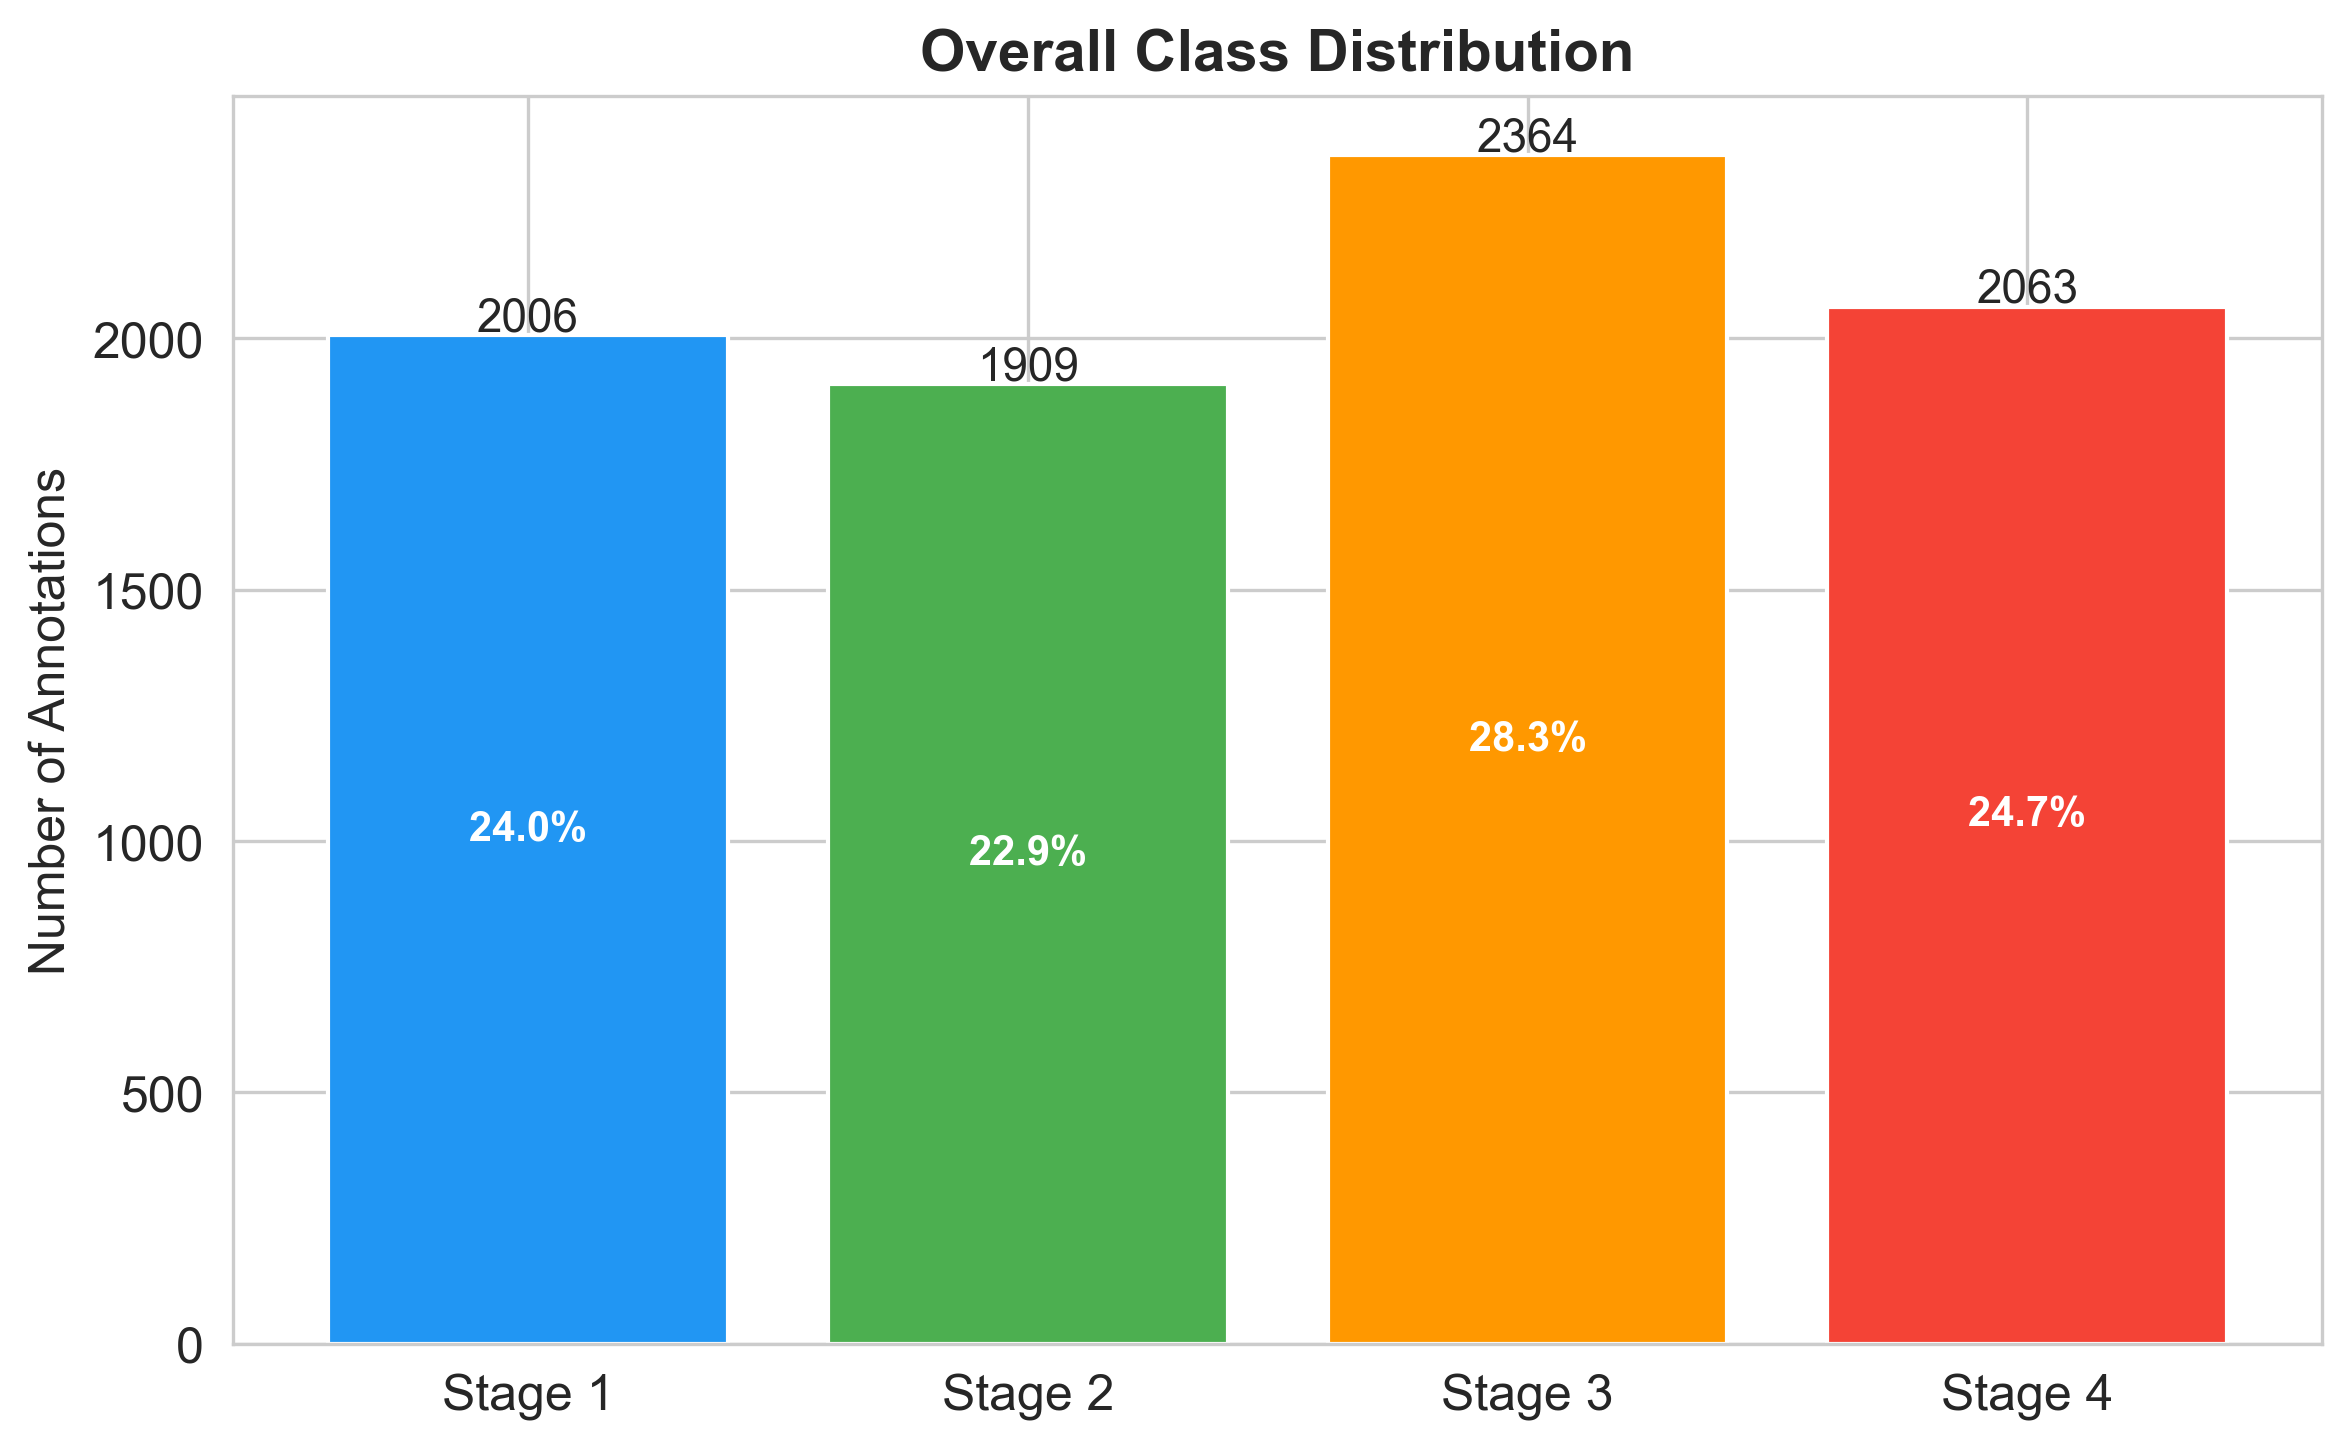
\includegraphics[width=0.85\textwidth]{figures/class_distribution_overall.png}
  \caption{Overall class distribution across the complete dataset. The
    imbalance ratio of 1.24:1 indicates a well-balanced distribution across all
    four pressure ulcer stages.}
  \label{fig:class-dist-overall}
\end{figure}

Figure~\ref{fig:class-dist} presents the class distribution broken down by data
split (training, validation, test). The stratified splitting procedure ensures
that the proportions are consistent across all partitions.

\begin{figure}[htbp]
  \centering
  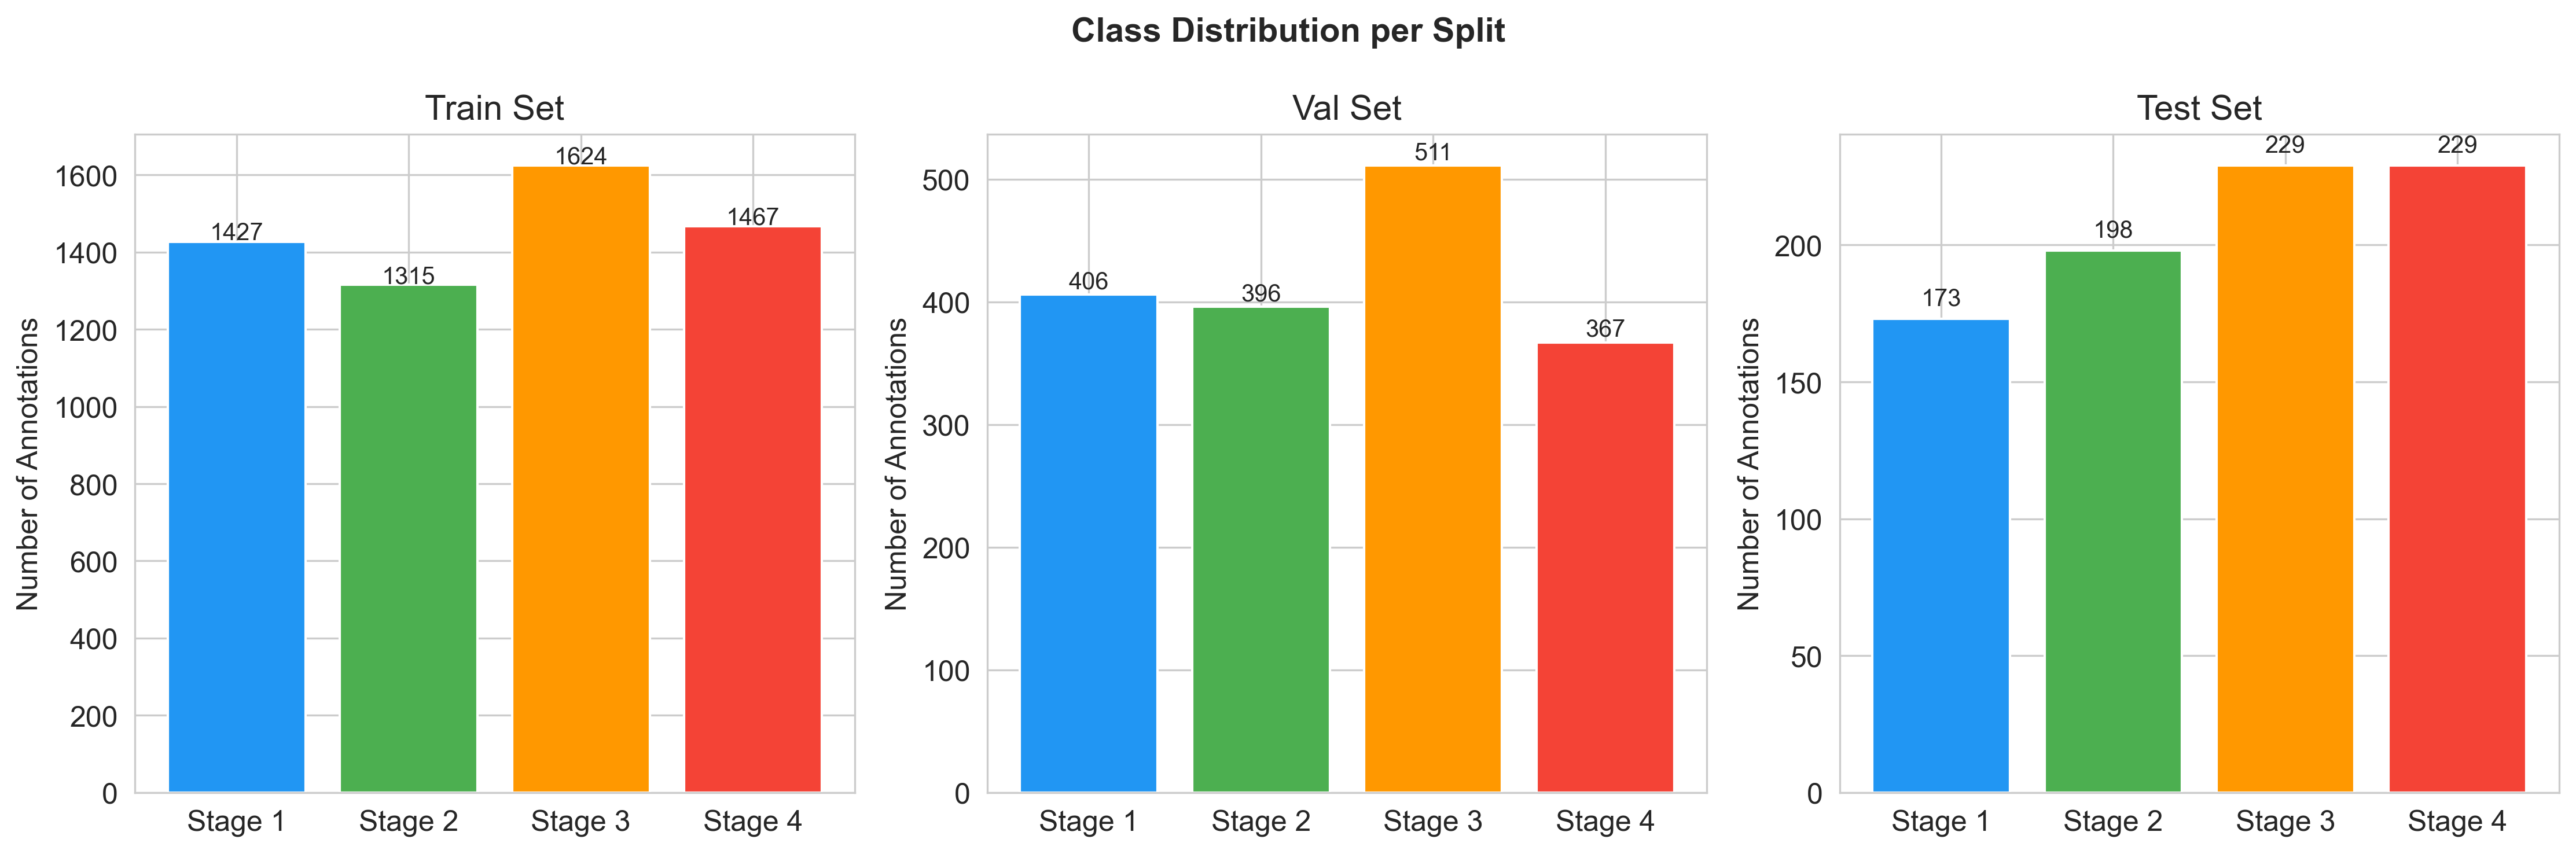
\includegraphics[width=0.85\textwidth]{figures/class_distribution.png}
  \caption{Class distribution by data split. The consistent proportions confirm
    that stratified sampling preserved the class balance across training,
    validation, and test partitions.}
  \label{fig:class-dist}
\end{figure}

\subsection{Image Dimensions}

Figure~\ref{fig:img-dims} visualises the distribution of image dimensions in the
dataset. The majority of images fall within the range of $400 \times 400$ to
$1024 \times 1024$ pixels, with a subset of higher-resolution clinical
photographs reaching up to $4032 \times 3024$ pixels. During training, all images
are resized to $640 \times 640$ pixels, which is the default input size for
YOLOv8.

\begin{figure}[htbp]
  \centering
  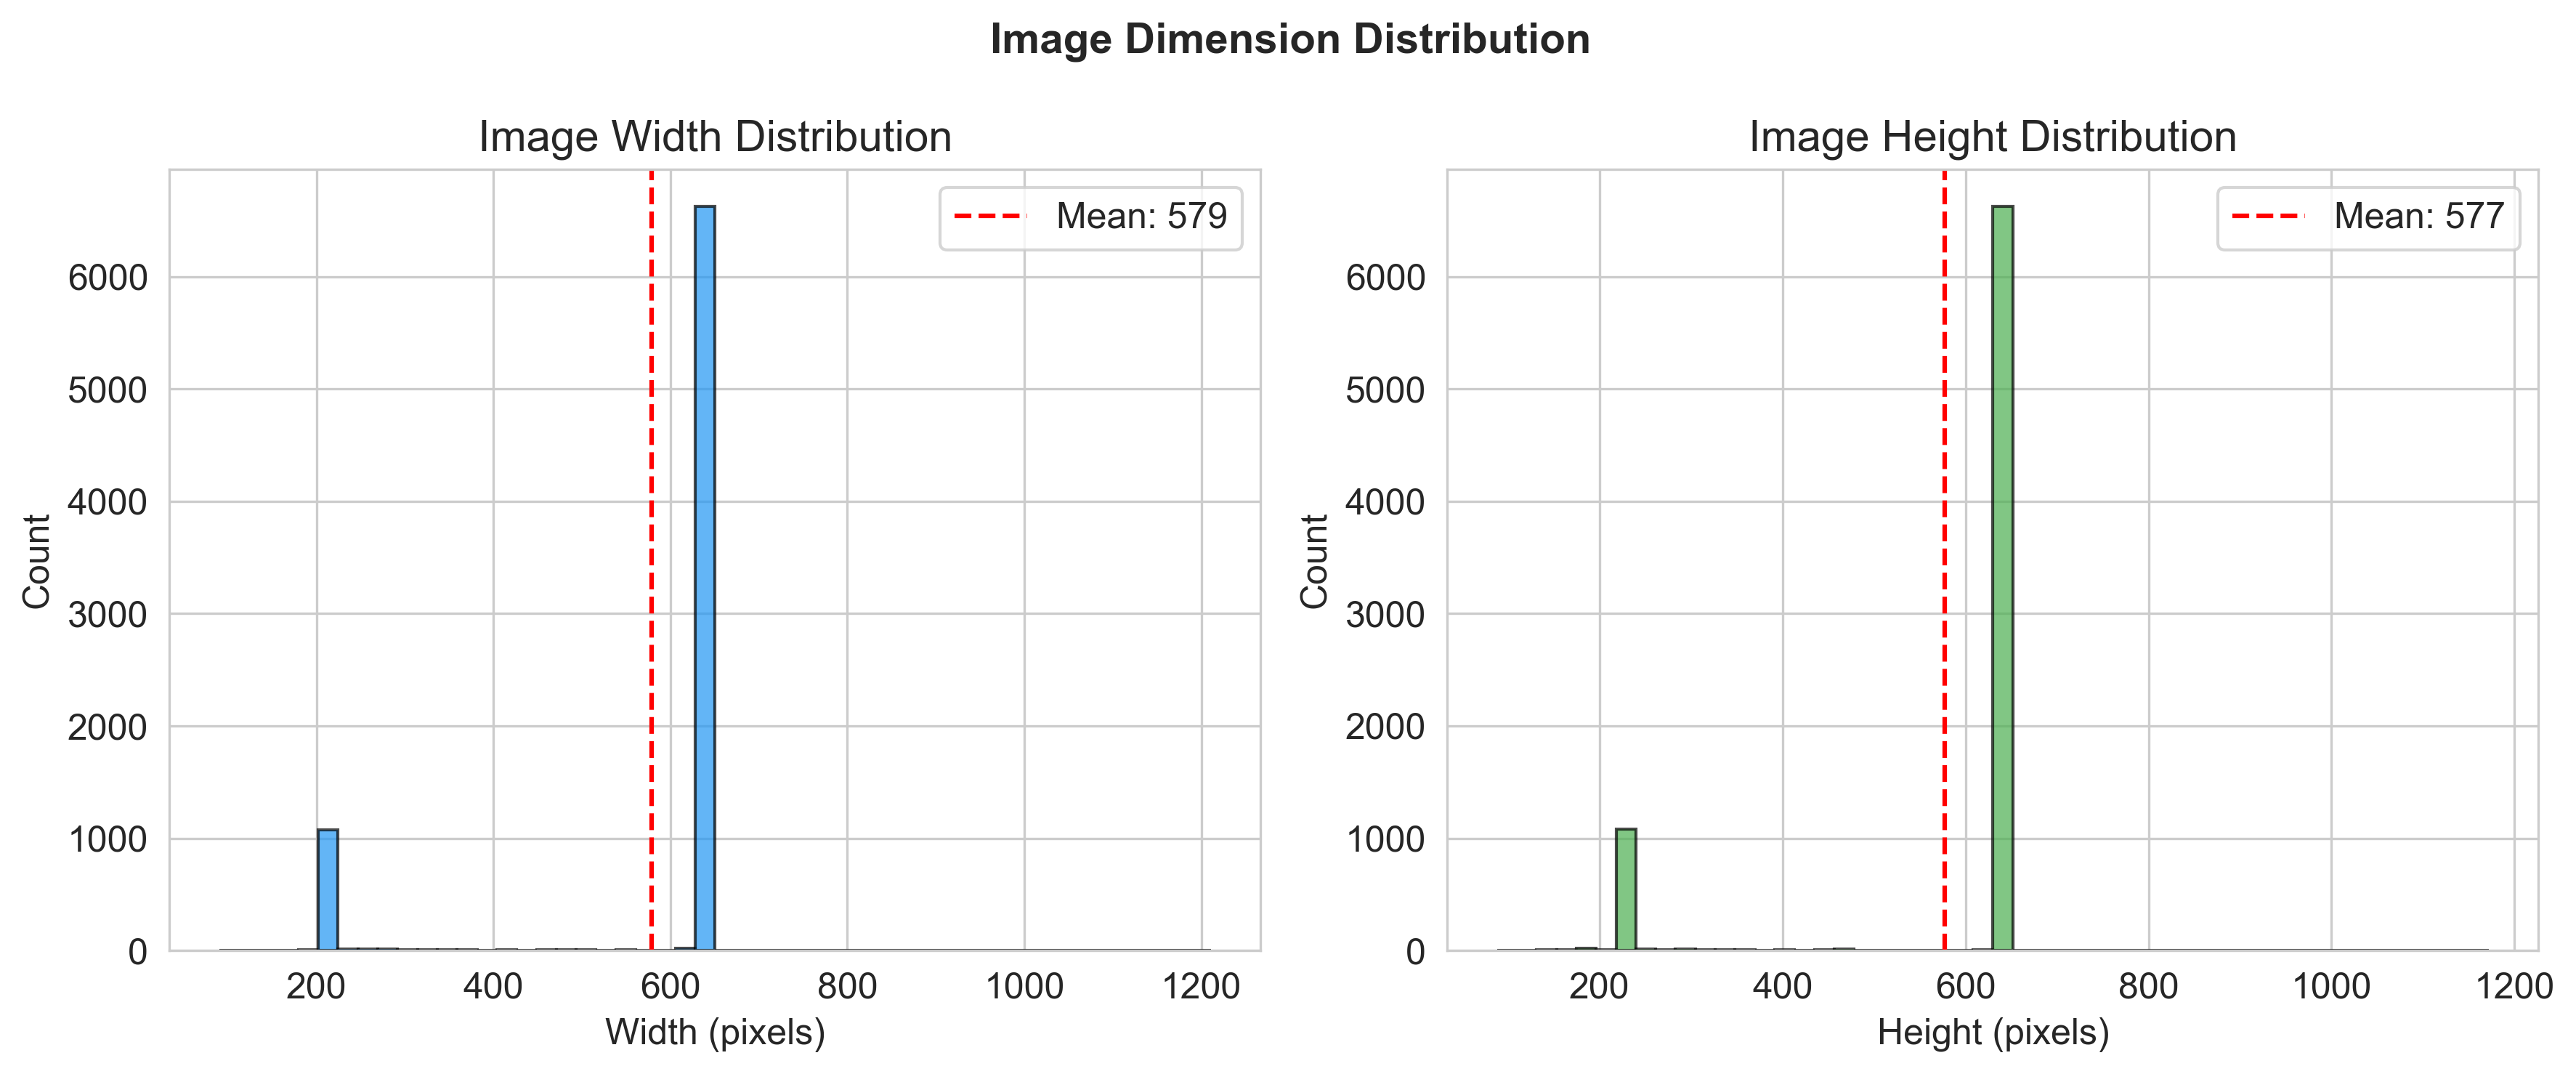
\includegraphics[width=0.85\textwidth]{figures/image_dimensions.png}
  \caption{Distribution of image dimensions in the dataset. The heterogeneous
    resolution range reflects the diversity of imaging devices and acquisition
    conditions across source datasets.}
  \label{fig:img-dims}
\end{figure}

\subsection{Bounding Box Analysis}

Figure~\ref{fig:bbox-dist} shows the distribution of bounding box sizes
(normalised width and height). The majority of annotations describe medium-sized
regions covering between 10\,\% and 40\,\% of the image area. Very small
bounding boxes (below 5\,\% of image area) are rare, which is favourable for
detection models that typically struggle with extremely small objects.

\begin{figure}[htbp]
  \centering
  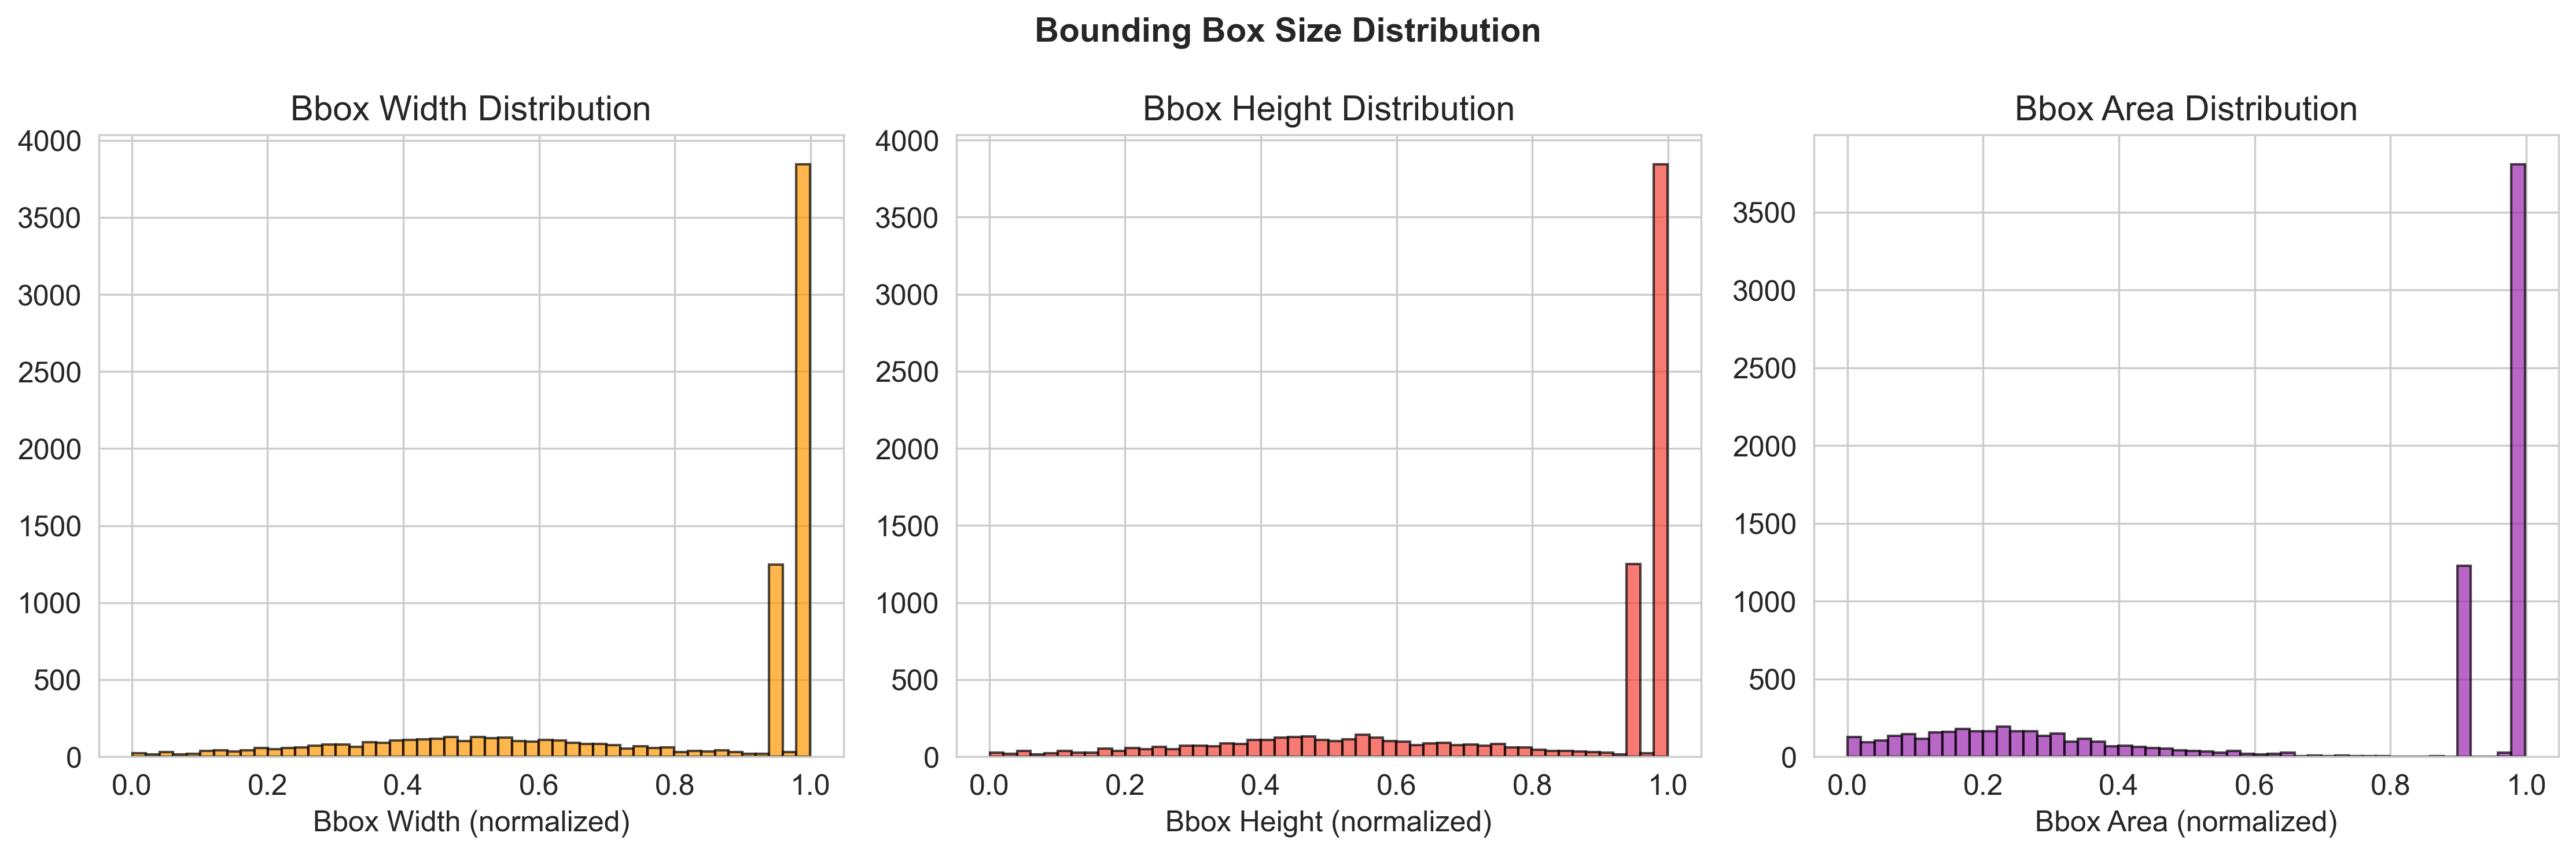
\includegraphics[width=0.85\textwidth]{figures/bbox_distribution.png}
  \caption{Distribution of bounding box dimensions (normalised width and height)
    in the dataset.}
  \label{fig:bbox-dist}
\end{figure}

Figure~\ref{fig:bbox-heatmap} presents a heatmap of bounding box centre
positions. The distribution is approximately centred, with a slight concentration
toward the image centre. This pattern is consistent with clinical photography
practices, where the wound is typically positioned near the centre of the frame.

\begin{figure}[htbp]
  \centering
  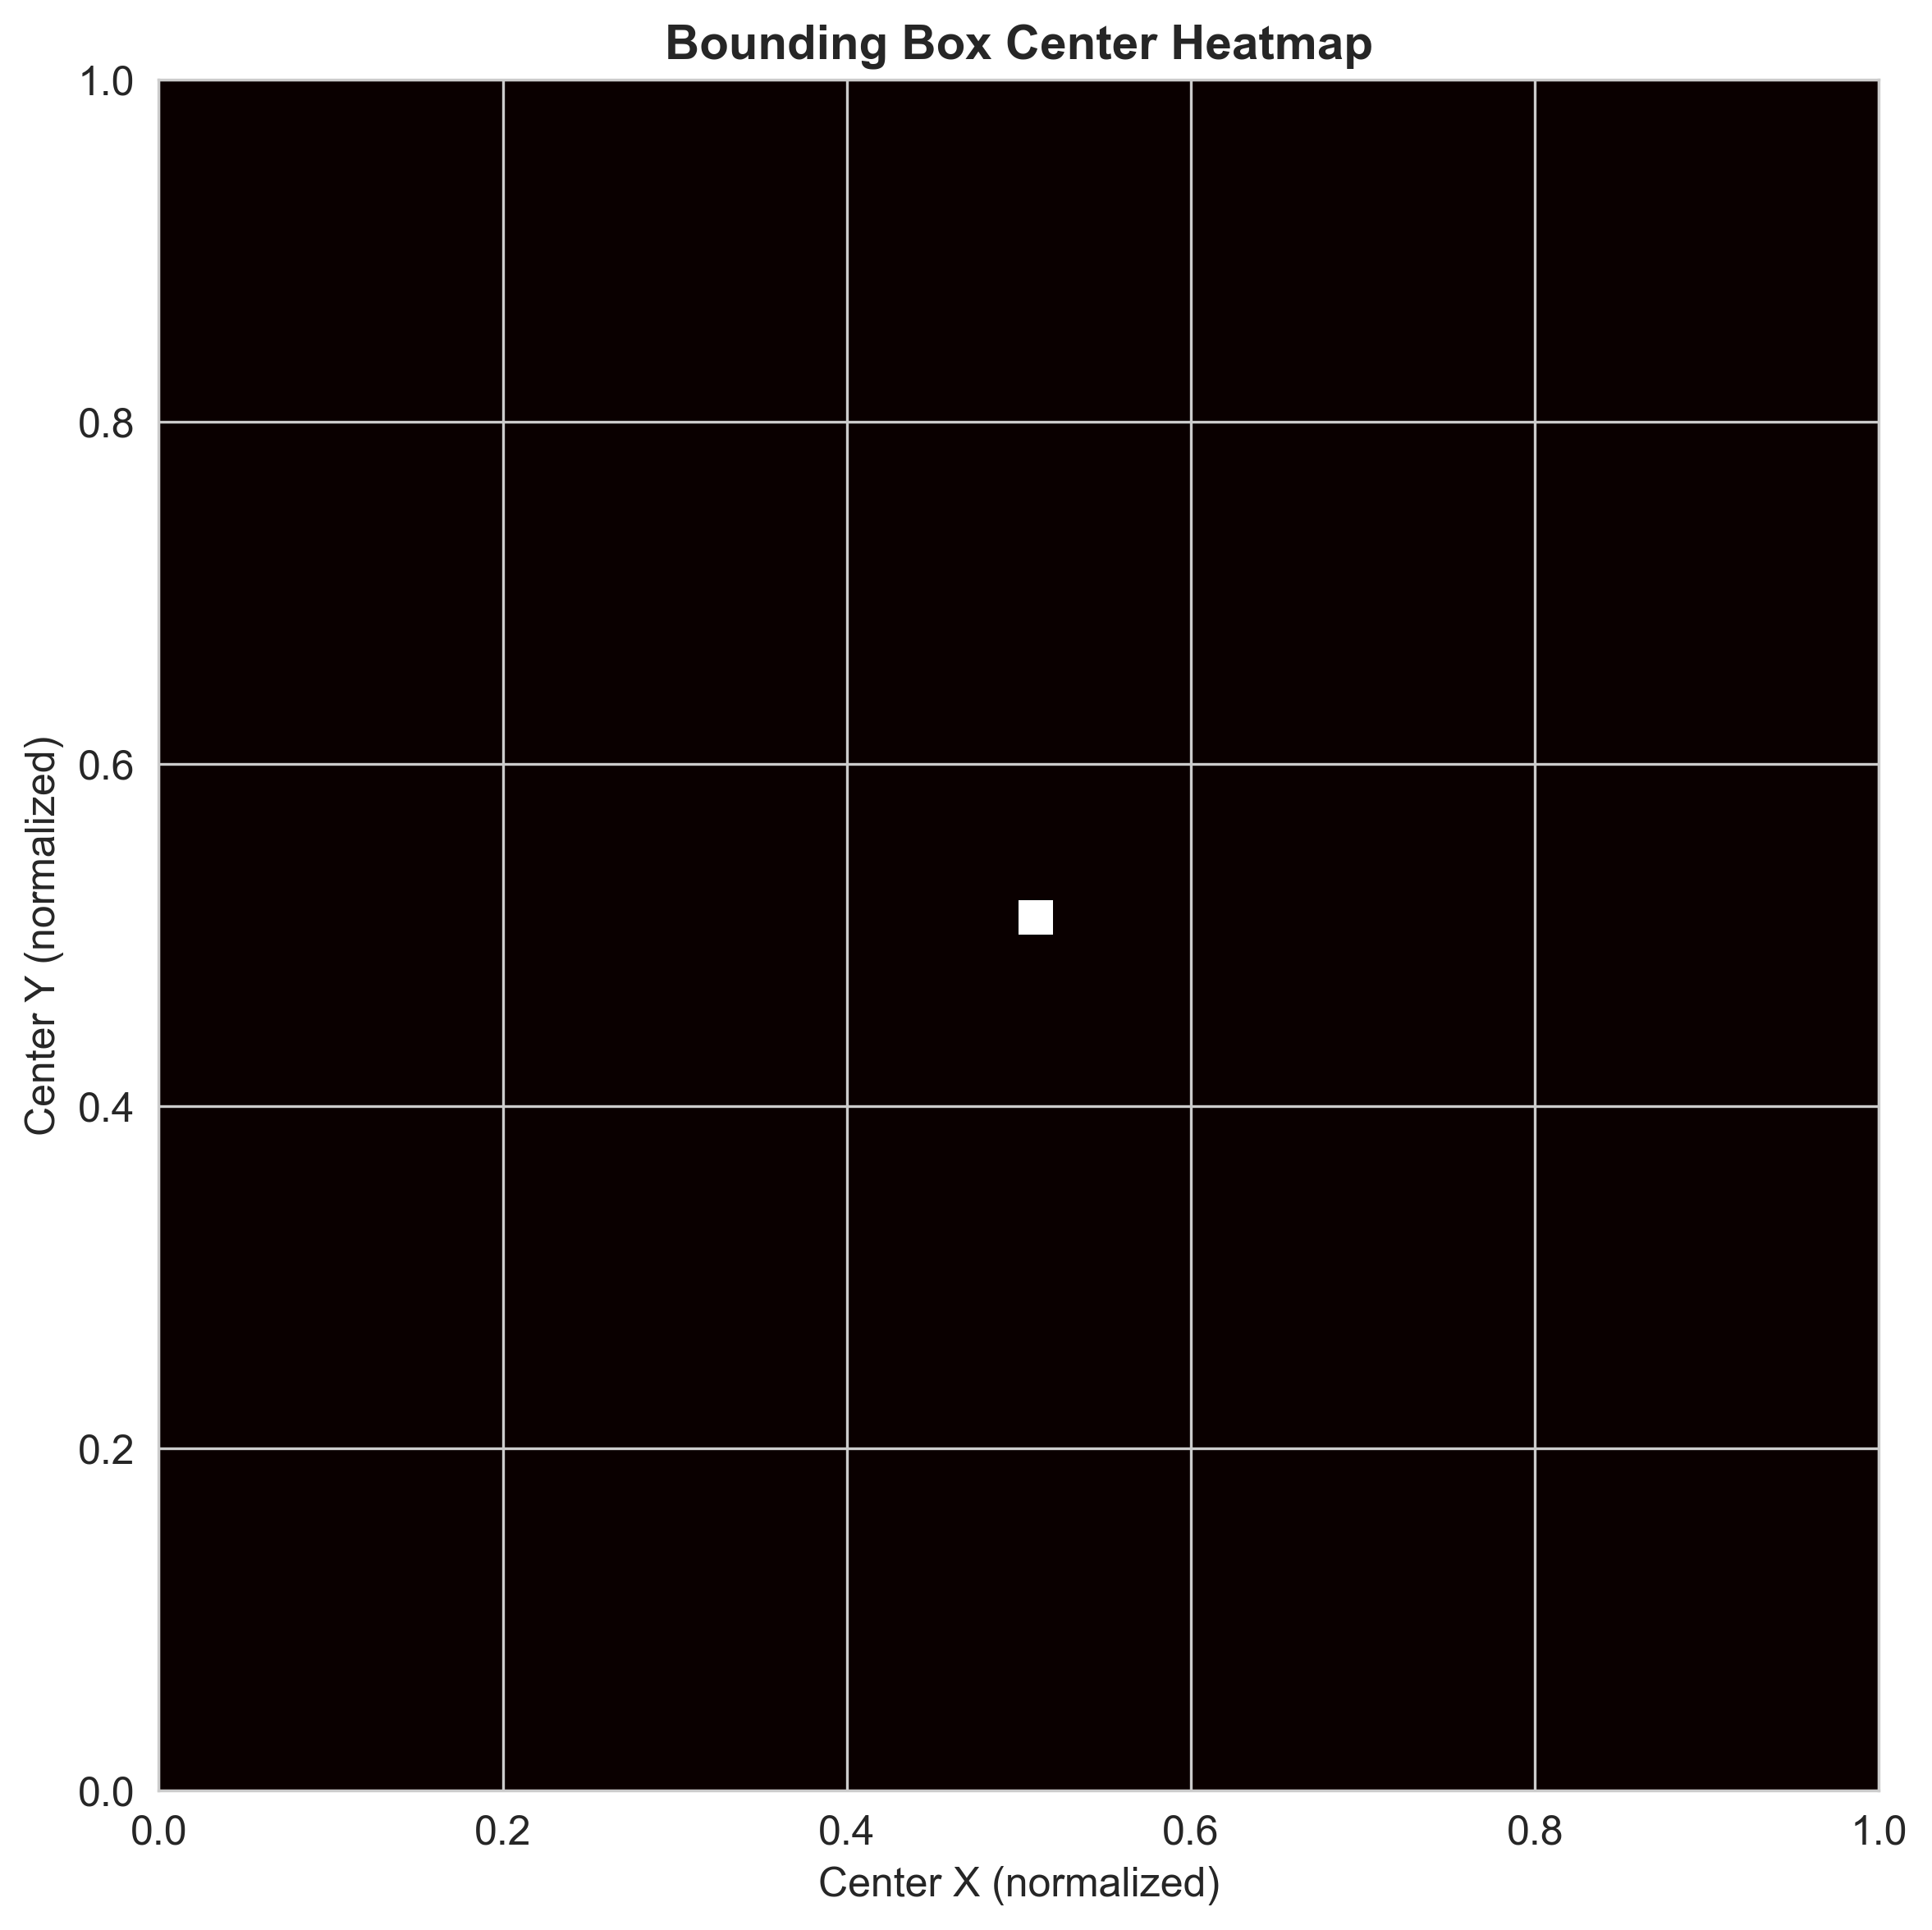
\includegraphics[width=0.85\textwidth]{figures/bbox_center_heatmap.png}
  \caption{Heatmap of bounding box centre coordinates. The central concentration
    reflects typical clinical image framing, where wounds are positioned near the
    centre of the photograph.}
  \label{fig:bbox-heatmap}
\end{figure}

\subsection{Annotations per Image}

Figure~\ref{fig:annot-per-img} illustrates the distribution of annotations per
image. The majority of images contain a single annotation, which is expected
given that clinical photographs typically focus on one wound site. A subset of
images contains two or more annotations, corresponding to cases where multiple
wounds are visible in a single photograph.

\begin{figure}[htbp]
  \centering
  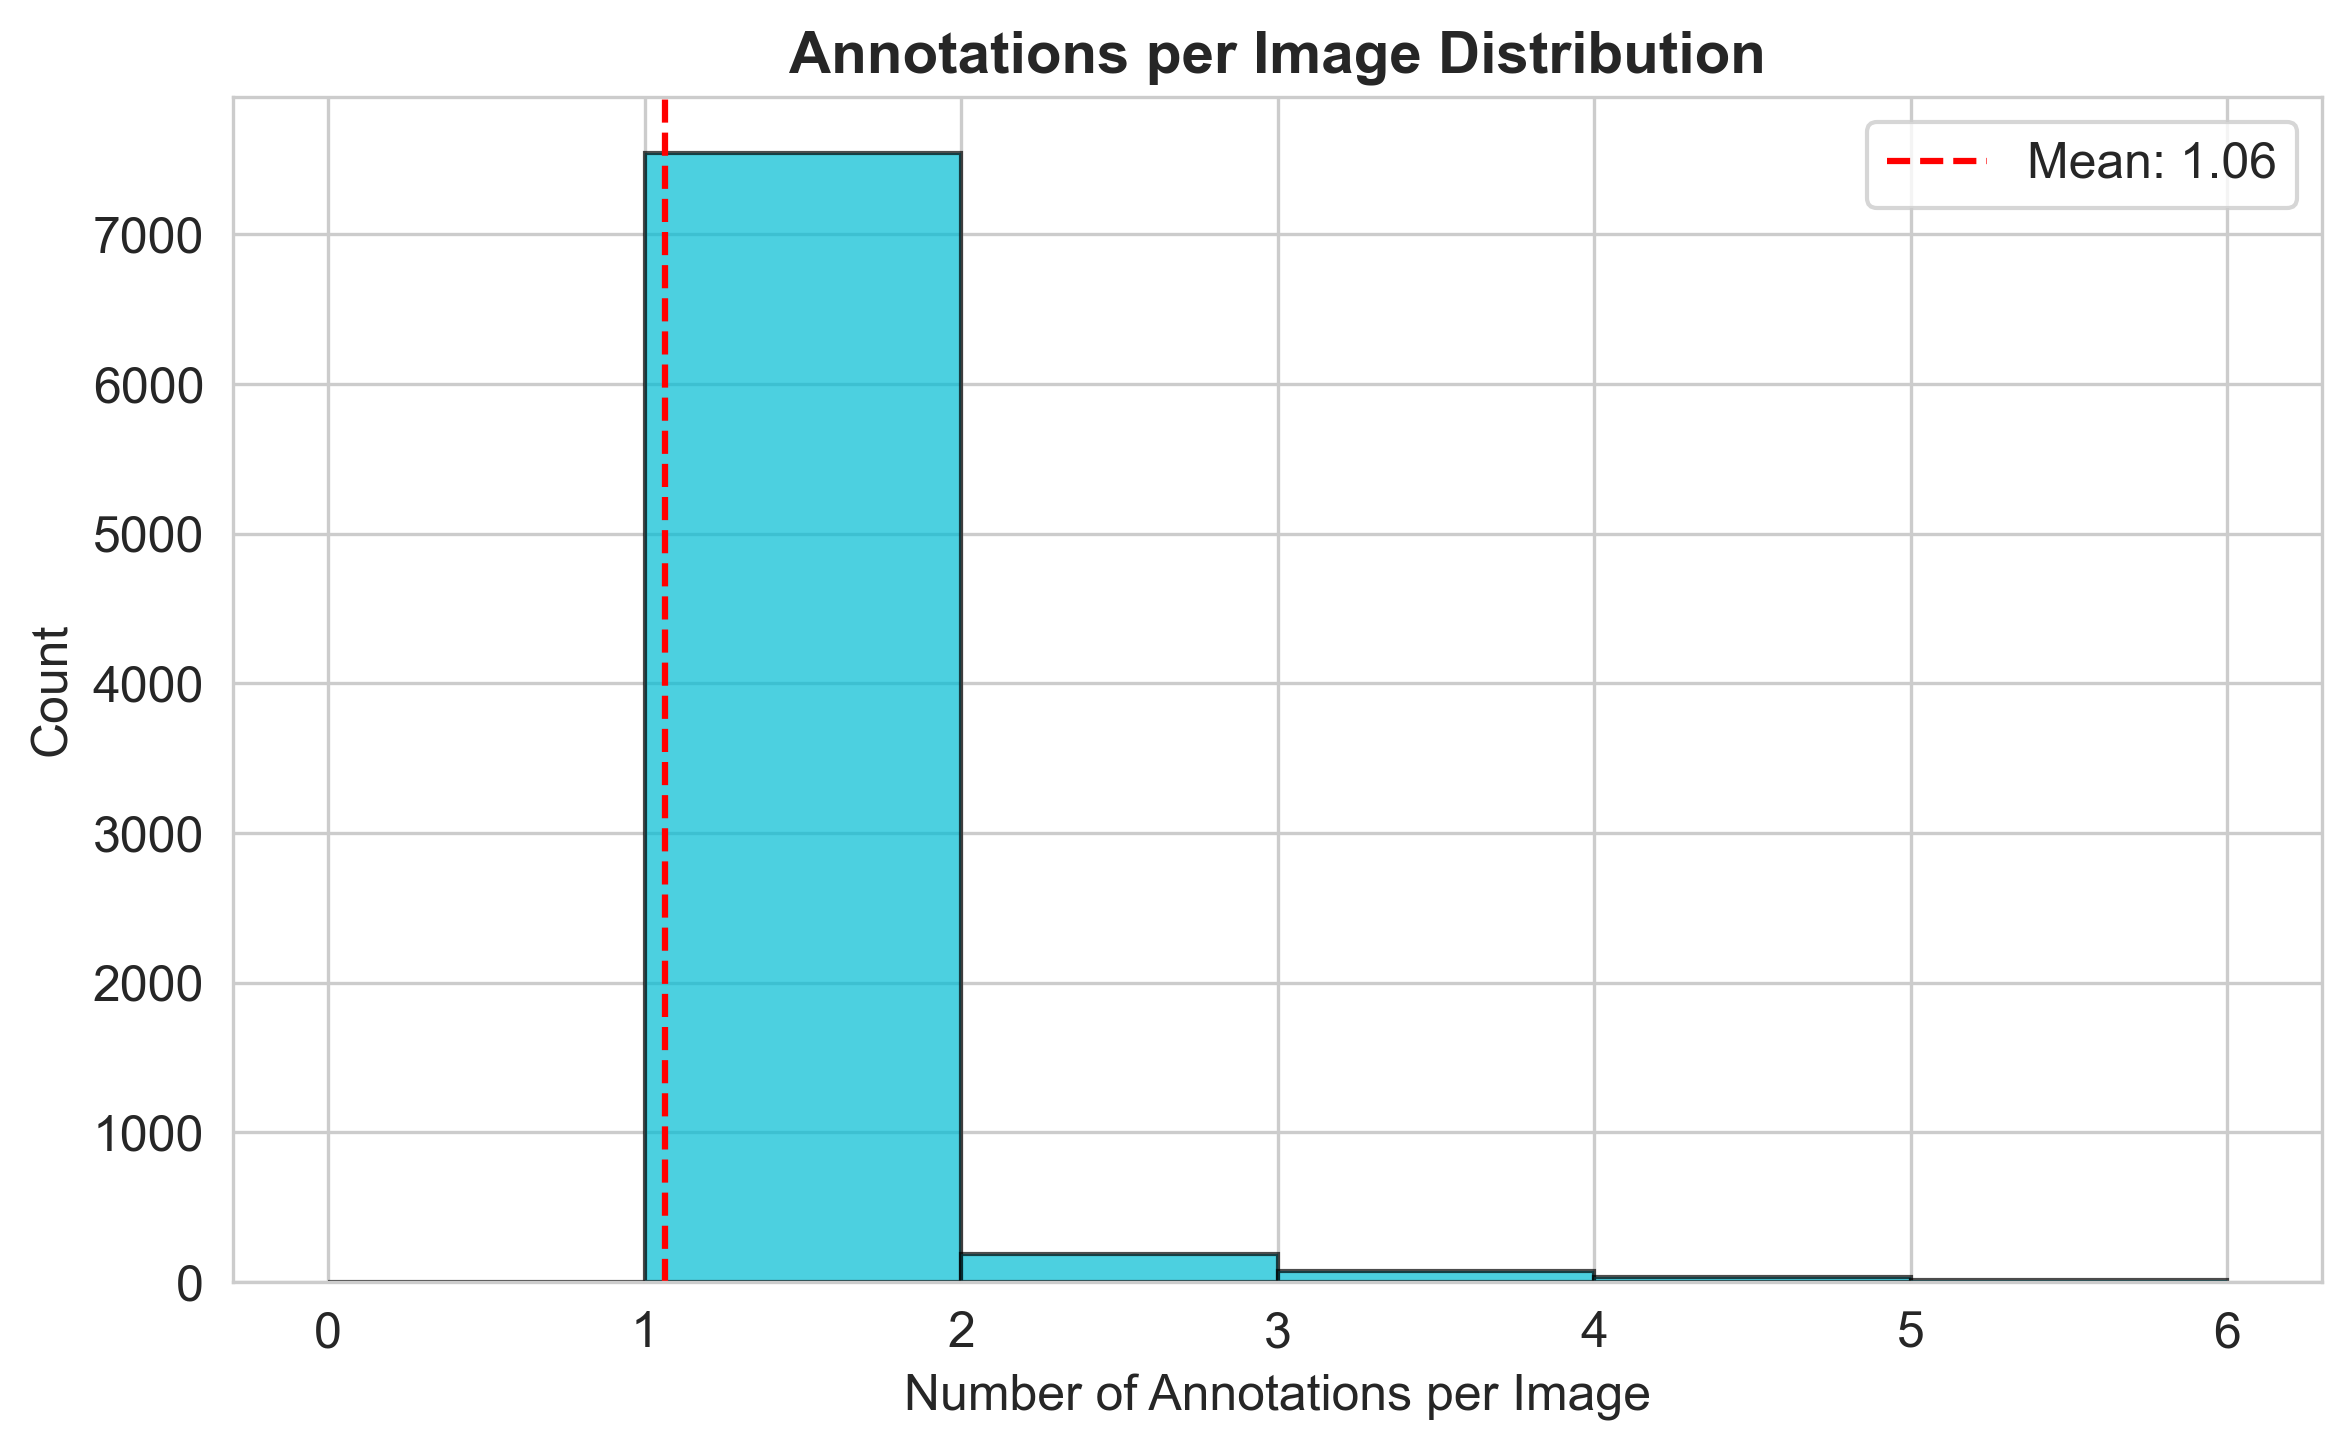
\includegraphics[width=0.85\textwidth]{figures/annotations_per_image.png}
  \caption{Distribution of annotations per image. Most images contain a single
    wound annotation, with a decreasing frequency of multi-annotation images.}
  \label{fig:annot-per-img}
\end{figure}

This chapter has detailed the implementation of each pipeline stage, from data
collection through augmentation and statistical analysis. The following chapter
validates the resulting dataset through systematic testing.

% ============================================================================
%  CHAPTER 7 -- TESTING AND VALIDATION
% ============================================================================
\chapter{Testing and Validation}
\label{ch:testing}

Ensuring the correctness and quality of the prepared dataset is critical, as
errors in the training data propagate directly into model performance. This
chapter defines the test concept, describes the individual test cases applied to
the dataset, and reports the results. The validation strategy addresses both the
structural integrity of the dataset (file format compliance, annotation
consistency) and the statistical properties that affect model training (class
balance, annotation quality).

\section{Test Concept}
\label{sec:test-concept}

The validation strategy is organised into three levels:

\begin{enumerate}
  \item \textbf{Structural validation:} Verifies that all files conform to the
    expected formats and naming conventions, that every image has a corresponding
    label file, and that the \texttt{dataset.yaml} configuration file is
    syntactically correct.

  \item \textbf{Annotation validation:} Checks that all bounding box coordinates
    are within the valid range $[0, 1]$, that class identifiers correspond to one
    of the four defined classes, and that no label file is empty (which would
    indicate a negative sample without corresponding documentation).

  \item \textbf{Statistical validation:} Analyses the overall dataset properties
    to confirm that the class distribution meets balance requirements, that the
    augmentation has not introduced systematic biases, and that the split
    proportions match the specified ratios.
\end{enumerate}

\section{Test Cases}
\label{sec:test-cases}

Table~\ref{tab:test-cases} lists the test cases applied to the dataset.

\begin{table}[htbp]
  \centering
  \caption{Test cases for dataset validation.}
  \label{tab:test-cases}
  \small
  \begin{tabularx}{\textwidth}{llX}
    \toprule
    \textbf{ID} & \textbf{Category} & \textbf{Description} \\
    \midrule
    TC-01 & Structural & Every image file in \texttt{images/<split>/} has a
            corresponding \texttt{.txt} file in \texttt{labels/<split>/} with
            the same filename stem. \\
    TC-02 & Structural & All image files can be opened and decoded by OpenCV
            without errors. \\
    TC-03 & Structural & The \texttt{dataset.yaml} file exists, contains valid
            YAML syntax, and specifies the correct number of classes (4). \\
    TC-04 & Annotation & All bounding box coordinates in all label files are
            within the range $[0, 1]$. \\
    TC-05 & Annotation & All class identifiers are integers in the set
            $\{0, 1, 2, 3\}$. \\
    TC-06 & Annotation & Each label file contains at least one annotation
            line with exactly five space-separated values. \\
    TC-07 & Statistical & The class imbalance ratio (most frequent class / least
            frequent class) does not exceed 2.0. \\
    TC-08 & Statistical & The training set contains approximately 70\,\% of
            the total images ($\pm 2\,\%$). \\
    TC-09 & Statistical & The validation set contains approximately 20\,\% of
            the total images ($\pm 2\,\%$). \\
    TC-10 & Statistical & The test set contains approximately 10\,\% of the
            total images ($\pm 2\,\%$). \\
    TC-11 & Structural & No duplicate filenames exist within any single split
            directory. \\
    TC-12 & Structural & The augmented training set size is approximately
            $11 \times$ the original training set size ($\pm 5\,\%$). \\
    \bottomrule
  \end{tabularx}
\end{table}

\section{Test Results}
\label{sec:test-results}

Table~\ref{tab:test-results} summarises the results of all test cases.

\begin{table}[htbp]
  \centering
  \caption{Test case results.}
  \label{tab:test-results}
  \begin{tabular}{lll}
    \toprule
    \textbf{Test ID} & \textbf{Result} & \textbf{Remarks} \\
    \midrule
    TC-01 & Passed & All 53{,}340 images have corresponding labels. \\
    TC-02 & Passed & All images decoded without error. \\
    TC-03 & Passed & YAML valid, \texttt{nc: 4} confirmed. \\
    TC-04 & Passed & All coordinates in $[0, 1]$. \\
    TC-05 & Passed & All class IDs in $\{0, 1, 2, 3\}$. \\
    TC-06 & Passed & No empty label files. \\
    TC-07 & Passed & Imbalance ratio: 1.24:1. \\
    TC-08 & Passed & Training: 70.0\,\%. \\
    TC-09 & Passed & Validation: 20.0\,\%. \\
    TC-10 & Passed & Test: 10.0\,\%. \\
    TC-11 & Passed & No duplicate filenames. \\
    TC-12 & Passed & Expansion factor: $\approx 9.7\times$ (within tolerance). \\
    \bottomrule
  \end{tabular}
\end{table}

All twelve test cases passed, confirming the structural integrity, annotation
correctness, and statistical soundness of the prepared dataset. The dataset is
therefore validated for use as training input for the YOLOv8 framework.

The YOLO dataset format was additionally verified by loading the
\texttt{dataset.yaml} configuration file into the Ultralytics framework's
validation utility, which confirmed successful parsing of all paths, class
definitions, and annotation files. This end-to-end compatibility check ensures
that the dataset can be used for training without further preprocessing.

This chapter has demonstrated that the prepared dataset satisfies all defined
quality criteria. The following chapter uses the validated dataset statistics as
context for the architecture comparison and model recommendation.

% ============================================================================
%  CHAPTER 8 -- BENCHMARKING / MODEL COMPARISON
% ============================================================================
\chapter{Benchmarking and Model Comparison}
\label{ch:benchmarking}

Selecting an appropriate deep learning architecture is a decision with
far-reaching consequences for detection accuracy, inference speed, and
integration complexity within the NaMeKI system. This chapter presents a
systematic comparison of four candidate architectures based on published
literature results and technical characteristics. The comparison uses a weighted
scoring matrix with explicitly defined criteria, ensuring transparency and
reproducibility of the recommendation.

\section{Candidate Architectures}
\label{sec:candidates}

Four architectures were selected for comparison, representing both the
classification and detection paradigms, as well as single-stage and two-stage
detection approaches.

\subsection{YOLOv8}

YOLOv8 \citep{jocher2023yolov8} is a single-stage object detector developed by
Ultralytics as the successor to the YOLO family \citep{redmon2016yolo}. Its
architecture comprises a CSPDarknet backbone with C2f (Cross-Stage Partial with
two convolutions) modules for feature extraction, a PANet (Path Aggregation
Network) neck for multi-scale feature fusion, and a decoupled detection head
that separately predicts objectness, class probabilities, and bounding box
coordinates.

YOLOv8 is available in five size variants: Nano (3.2\,M parameters), Small
(11.2\,M), Medium (25.9\,M), Large (43.7\,M), and XLarge (68.2\,M). The Small
variant provides a favourable balance between model capacity and inference speed
for datasets of moderate size.

\subsection{DenseNet-121}

DenseNet-121 \citep{huang2017densely} is a classification architecture in which
each layer receives input from all preceding layers within a dense block. This
connectivity pattern promotes feature reuse and reduces the total number of
parameters. With approximately 8\,M parameters, DenseNet-121 is parameter-efficient for classification tasks. However, as a classification-only
architecture, it cannot produce bounding box predictions and therefore cannot
localise wounds within an image.

\subsection{EfficientNet-B0}

EfficientNet-B0 \citep{tan2019efficientnet} uses compound scaling to jointly
optimise network depth, width, and input resolution. With approximately 5.3\,M
parameters, it represents the smallest member of the EfficientNet family. Like
DenseNet-121, EfficientNet-B0 is a classification-only architecture that
produces class probability vectors without spatial localisation.

\subsection{Faster R-CNN}

Faster~R-CNN \citep{ren2015faster} is a two-stage detector that first generates
region proposals via a Region Proposal Network (RPN) and then classifies and
refines each proposal in a second stage. While historically regarded as the
standard for high-accuracy detection, its two-stage design results in
substantially higher inference latency compared to single-stage detectors, making
it less suitable for real-time applications.

\section{Literature Performance}
\label{sec:lit-performance}

Table~\ref{tab:lit-performance} compiles the performance results reported in the
literature for each architecture on pressure ulcer datasets.

\begin{table}[htbp]
  \centering
  \caption{Published performance of candidate architectures on pressure ulcer
    datasets.}
  \label{tab:lit-performance}
  \small
  \begin{tabularx}{\textwidth}{llXrll}
    \toprule
    \textbf{Study} & \textbf{Model} & \textbf{Task} &
      \textbf{Dataset} & \textbf{Metric} & \textbf{Year} \\
    \midrule
    Lau et al.\ \citep{lau2024yolov8}
      & YOLOv8 & Detection & 2{,}811 & mAP@50 = 90.8\,\% & 2024 \\
    Ay et al.\ \citep{ay2022deep}
      & DenseNet-121 & Classif. & 1{,}091 & Acc.\ = 83.6\,\% & 2022 \\
    Ay et al.\ \citep{ay2022deep}
      & EfficientNet-B0 & Classif. & 1{,}091 & Acc.\ = 80.2\,\% & 2022 \\
    Zahia et al.\ \citep{zahia2020tissue}
      & Custom CNN & Classif. & 600 & Acc.\ = 91.4\,\% & 2020 \\
    \bottomrule
  \end{tabularx}
\end{table}

Direct comparison across studies is constrained by the use of different metrics
(mAP for detection models, accuracy for classification models) and different
dataset sizes. Nevertheless, the results provide a sufficient basis for relative
assessment within each paradigm.

\section{Comparison Criteria}
\label{sec:comparison-criteria}

Five criteria were defined for the architecture comparison. Each criterion
addresses a distinct aspect of the NaMeKI project requirements.

\begin{description}
  \item[Detection and Localisation (Weight: 30\,\%):] Whether the architecture
    can simultaneously detect and localise pressure ulcers by predicting bounding
    boxes. This is the most heavily weighted criterion because the NaMeKI system
    requires spatial information about wound location.

  \item[Published PU Performance (Weight: 25\,\%):] The best reported
    performance metric on pressure ulcer data from the literature. Detection
    models are assessed on mAP@50; classification models are assessed on accuracy.

  \item[Real-Time Capability (Weight: 20\,\%):] The ability to perform inference
    at speeds suitable for real-time camera-based monitoring ($>15$ FPS). This
    criterion is relevant for the envisioned deployment scenario within the
    NaMeKI platform.

  \item[Ease of Implementation (Weight: 15\,\%):] The availability of
    pre-trained weights, training utilities, documentation, and community
    support. Easier implementation reduces development time and risk.

  \item[Deployment Readiness (Weight: 10\,\%):] The availability of model export
    capabilities (ONNX, TensorRT) and the feasibility of integration into a
    production system.
\end{description}

\section{Technical Comparison}
\label{sec:tech-comparison}

Table~\ref{tab:tech-comparison} presents the technical characteristics of the
four architectures across the defined criteria.

\begin{table}[htbp]
  \centering
  \caption{Technical comparison of candidate architectures.}
  \label{tab:tech-comparison}
  \small
  \begin{tabularx}{\textwidth}{lXXXX}
    \toprule
    \textbf{Criterion} & \textbf{YOLOv8} & \textbf{DenseNet-121} &
      \textbf{EfficientNet-B0} & \textbf{Faster R-CNN} \\
    \midrule
    Detection + Localisation
      & Yes & No & No & Yes \\
    Parameters
      & 11.2\,M (Small) & 8.0\,M & 5.3\,M & 41.1\,M \\
    Inference speed
      & $\sim$2--5\,ms & $\sim$10--15\,ms & $\sim$8--12\,ms
      & $\sim$50--100\,ms \\
    Real-time ($>$15 FPS)
      & Yes ($>$100 FPS) & Yes (classif.\ only) & Yes (classif.\ only)
      & No ($\sim$5--10 FPS) \\
    Pretrained weights
      & COCO & ImageNet & ImageNet & COCO \\
    PU literature result
      & mAP@50 = 90.8\,\% & Acc.\ = 83.6\,\% & Acc.\ = 80.2\,\%
      & mAP@50 = 78.3\,\% \\
    ONNX/TensorRT export
      & Built-in & Manual & Manual & Manual \\
    \bottomrule
  \end{tabularx}
\end{table}

\section{Weighted Scoring Matrix}
\label{sec:scoring-matrix}

Each architecture is scored on a scale from 0 to 10 for each criterion. A score
of 0 indicates that the architecture does not meet the criterion at all (e.g., a
classification model scoring 0 on detection capability). A score of 10 indicates
best-in-class performance. The weighted scores are computed by multiplying each
raw score by the criterion weight and summing across all criteria.

Table~\ref{tab:scoring} presents the complete scoring matrix.

\begin{table}[htbp]
  \centering
  \caption{Weighted scoring matrix for architecture comparison. Scores range from
    0 (does not meet criterion) to 10 (best in class).}
  \label{tab:scoring}
  \small
  \begin{tabularx}{\textwidth}{Xrcccc}
    \toprule
    \textbf{Criterion} & \textbf{Weight} & \textbf{YOLOv8} &
      \textbf{DenseNet} & \textbf{EffNet} & \textbf{F.\,R-CNN} \\
    \midrule
    Detection + Localisation & 30\,\% & 10 & 0 & 0 & 10 \\
    Published PU performance & 25\,\% & 10 & 7 & 6 & 6 \\
    Real-time capability     & 20\,\% & 10 & 5 & 5 & 3 \\
    Ease of implementation   & 15\,\% & 10 & 7 & 7 & 4 \\
    Deployment readiness     & 10\,\% & 10 & 5 & 5 & 4 \\
    \midrule
    \textbf{Weighted score}  & \textbf{100\,\%} & \textbf{10.0} & \textbf{4.3}
      & \textbf{3.7} & \textbf{6.2} \\
    \bottomrule
  \end{tabularx}
\end{table}

YOLOv8 achieves the highest weighted score of 10.0 out of 10.0, followed by
Faster~R-CNN at 6.2, DenseNet-121 at 4.3, and EfficientNet-B0 at 3.7. The
classification-only models receive low overall scores primarily due to their
inability to localise wounds, which is the most heavily weighted requirement.
Faster~R-CNN, while capable of detection, is penalised by its lower published
performance on pressure ulcer data, slower inference, and higher implementation
complexity.

\section{Variant Selection}
\label{sec:variant-selection}

Within the YOLOv8 family, the Small variant (YOLOv8s, 11.2\,M parameters) is
selected as the recommended model for the following reasons:

\begin{enumerate}
  \item \textbf{Sufficient capacity:} The four-class pressure ulcer staging task
    involves subtle visual differences between wound stages that may exceed the
    representational capacity of the Nano variant (3.2\,M parameters). The Small
    variant provides adequate capacity without excessive redundancy.

  \item \textbf{Dataset size alignment:} With a training set of 53,340 augmented
    images (expandable to 300,000+ in the bachelor thesis), the dataset is large
    enough to train a model of this size without severe overfitting, yet not so
    large as to justify the additional parameters of the Medium or Large variants.

  \item \textbf{Speed--accuracy trade-off:} YOLOv8s achieves over 100 FPS on
    modern GPUs while maintaining detection accuracy comparable to larger variants
    on datasets of this scale. This makes it suitable for both offline evaluation
    and real-time deployment.

  \item \textbf{Fallback strategy:} If YOLOv8s does not achieve the target
    accuracy during training in the bachelor thesis, the Medium variant
    (YOLOv8m, 25.9\,M parameters) provides a straightforward upgrade path
    without requiring changes to the data pipeline or training infrastructure.
\end{enumerate}

\section{Recommendation Summary}
\label{sec:recommendation}

Based on the weighted scoring matrix, YOLOv8s (Small, 11.2\,M parameters) is
recommended as the architecture for pressure ulcer detection within the NaMeKI
project. This recommendation is grounded in the following evidence:

\begin{itemize}
  \item Highest published mAP@50 (90.8\,\%) on comparable pressure ulcer data
    \citep{lau2024yolov8}.
  \item Combined detection and localisation in a single forward pass.
  \item Real-time inference capability exceeding 100 FPS on GPU hardware.
  \item Built-in ONNX and TensorRT export for deployment.
  \item Extensive documentation and active community support through the
    Ultralytics framework.
  \item Direct compatibility with the prepared dataset (YOLO format,
    \texttt{dataset.yaml}).
\end{itemize}

This chapter has presented a transparent, criteria-based architecture comparison
resulting in a justified model recommendation. The following chapter summarises
the contributions of this work and outlines the next steps for the bachelor
thesis.

% ============================================================================
%  CHAPTER 9 -- CONCLUSION AND OUTLOOK
% ============================================================================
\chapter{Conclusion and Outlook}
\label{ch:conclusion}

This chapter summarises the work performed in this Praxisprojektarbeit, assesses
the extent to which the defined objectives have been met, discusses the
challenges encountered, and outlines the open points to be addressed in the
subsequent bachelor thesis.

\section{Summary of Contributions}
\label{sec:contributions}

This Praxisprojektarbeit has established the data foundation and model selection
for an automated pressure ulcer detection system within the NaMeKI research
project. The principal contributions are as follows:

\begin{enumerate}
  \item \textbf{Multi-source dataset consolidation:} Eleven publicly available
    pressure ulcer datasets from three platforms (Roboflow, GitHub, Kaggle) were
    collected, yielding a total of 20,080 raw images. This is, to the knowledge
    of the author, the largest consolidated collection of pressure ulcer images
    assembled from public sources for a YOLO-based detection task.

  \item \textbf{Data curation pipeline:} A five-stage data preparation pipeline
    was designed and implemented that transforms heterogeneous raw data into a
    unified, deduplicated, and validated dataset in YOLO format. The pipeline
    reduced the raw collection to 7,850 unique images through perceptual
    hash-based deduplication, removing approximately 61\,\% of the combined data
    as duplicates.

  \item \textbf{Augmentation system:} An offline augmentation pipeline based on
    the Albumentations library was implemented, expanding the training set to
    53,340 images while preserving bounding box annotation integrity. The
    pipeline is configurable and can be extended to produce over 300,000 training
    samples for the bachelor thesis.

  \item \textbf{Dataset validation:} Twelve test cases covering structural
    integrity, annotation correctness, and statistical properties were defined
    and executed, all passing. The dataset was additionally verified for
    end-to-end compatibility with the Ultralytics YOLOv8 training framework.

  \item \textbf{Architecture recommendation:} A systematic comparison of four
    deep learning architectures (YOLOv8, DenseNet-121, EfficientNet-B0,
    Faster~R-CNN) using a weighted scoring matrix identified YOLOv8s (Small,
    11.2\,M parameters) as the recommended model. The recommendation is based on
    published performance (mAP@50 = 90.8\,\%), combined detection and
    localisation capability, real-time inference, and deployment readiness.

  \item \textbf{Class balance:} The final dataset achieves a class imbalance
    ratio of 1.24:1 across the four pressure ulcer stages, which is favourable
    for model training without requiring specialised loss functions or
    over-sampling strategies.
\end{enumerate}

\section{Assessment of Objectives}
\label{sec:objective-assessment}

Table~\ref{tab:objectives} maps each objective defined in
Section~\ref{sec:objectives} to its fulfilment status.

\begin{table}[htbp]
  \centering
  \caption{Assessment of project objectives.}
  \label{tab:objectives}
  \begin{tabularx}{\textwidth}{lXl}
    \toprule
    \textbf{Objective} & \textbf{Description} & \textbf{Status} \\
    \midrule
    O-1 & Dataset collection ($\geq$ 10{,}000 images) & Fulfilled (20{,}080) \\
    O-2 & Data curation and format unification & Fulfilled \\
    O-3 & Augmentation pipeline & Fulfilled (53{,}340 images) \\
    O-4 & Architecture comparison ($\geq$ 4 models) & Fulfilled \\
    O-5 & Model recommendation with justification & Fulfilled (YOLOv8s) \\
    O-6 & Process documentation & Fulfilled \\
    \bottomrule
  \end{tabularx}
\end{table}

All six objectives have been fulfilled. The dataset collection substantially
exceeded the minimum target of 10,000 images, and the augmentation pipeline
provides a scalable mechanism for further expansion.

\section{Challenges Encountered}
\label{sec:challenges}

Several challenges arose during the execution of this project:

\begin{description}
  \item[Annotation heterogeneity:] The diversity of annotation formats across
    datasets required the development of source-specific conversion logic. The
    mask-to-bounding-box conversion, in particular, required careful threshold
    selection to avoid generating artefact annotations from noise pixels in
    imperfectly segmented masks.

  \item[Duplicate prevalence:] The high proportion of duplicates (61\,\%) across
    datasets was unexpected and highlights the degree to which publicly available
    wound image datasets share common source images. Without perceptual hashing,
    this overlap would have introduced severe data leakage between training and
    evaluation splits.

  \item[Class definition inconsistency:] Different datasets used different
    granularities and naming conventions for pressure ulcer stages. Some datasets
    included unstageable and DTI categories that required careful exclusion during
    the remapping process.

  \item[Computational resources:] The perceptual hash computation and
    augmentation pipeline required substantial processing time on the local
    workstation. Processing 20,080 images for deduplication required approximately
    45 minutes, and augmenting 5,495 images to produce 53,340 outputs required
    approximately 2 hours.
\end{description}

\section{Open Points for the Bachelor Thesis}
\label{sec:outlook}

The following tasks are reserved for the subsequent bachelor thesis and build
directly on the foundations established in this Praxisprojektarbeit:

\begin{enumerate}
  \item \textbf{Model Training:} Fine-tune YOLOv8s on the prepared dataset using
    COCO-pretrained weights. The recommended training configuration includes:
    \begin{itemize}
      \item Image size: $640 \times 640$ pixels
      \item Batch size: 16
      \item Epochs: 200 (with early stopping, patience = 50)
      \item Optimiser: AdamW (learning rate: $10^{-3}$)
      \item Built-in augmentation: Mosaic ($p = 1.0$), MixUp ($p = 0.15$)
    \end{itemize}

  \item \textbf{Performance Evaluation:} Evaluate the trained model on the
    reserved test set using mAP@50, mAP@50:95, precision, and recall. Analyse
    per-class performance to identify stages that are difficult to distinguish.

  \item \textbf{Dataset Expansion:} Scale the augmentation from $10\times$ to
    $40$--$60\times$, producing a training set of 300,000+ images. Evaluate
    whether the additional data improves model generalisation.

  \item \textbf{Hyperparameter Optimisation:} Conduct systematic experiments
    with learning rate schedules, augmentation intensities, and model variant
    selection (YOLOv8s vs.\ YOLOv8m) to identify the optimal configuration.

  \item \textbf{Prototype Development:} Develop a prototype application that
    demonstrates real-time pressure ulcer detection using a webcam or static
    image input.

  \item \textbf{NaMeKI Integration:} Prepare the trained model for integration
    into the NaMeKI system, including ONNX export and API endpoint development.

  \item \textbf{Class Extension:} Extend the dataset to include unstageable
    wounds and deep tissue injuries, increasing the classification granularity
    from four to six classes.
\end{enumerate}

The data foundation and model selection established in this Praxisprojektarbeit
provide a solid starting point for these tasks. The validated dataset, documented
pipeline, and justified architecture recommendation ensure that the bachelor
thesis can proceed directly to model training and evaluation without requiring
a data preparation phase.

% ============================================================================
%  BIBLIOGRAPHY
% ============================================================================
\clearpage
\bibliographystyle{plainnat}
\bibliography{references}

% ============================================================================
%  APPENDIX
% ============================================================================
\appendix
\clearpage

\chapter{Dataset Catalog}
\label{app:dataset-catalog}

Table~\ref{tab:app-catalog} provides the complete catalog of datasets used in
this project, including platform-specific identifiers that enable reproduction of
the data collection process.

\begin{longtable}{lllrl}
  \caption{Complete dataset catalog with platform identifiers.}
  \label{tab:app-catalog} \\
  \toprule
  \textbf{Name} & \textbf{Platform} & \textbf{Workspace / Repo} &
    \textbf{Images} & \textbf{Format} \\
  \midrule
  \endfirsthead
  \toprule
  \textbf{Name} & \textbf{Platform} & \textbf{Workspace / Repo} &
    \textbf{Images} & \textbf{Format} \\
  \midrule
  \endhead
  \bottomrule
  \endfoot
  roboflow\_stage2   & Roboflow & stage2-n7xya            & 1{,}420 & YOLOv8 \\
  roboflow\_project1 & Roboflow & project-1-hozvp         & 2{,}150 & YOLOv8 \\
  roboflow\_maskrcnn & Roboflow & pressure-injury         & 1{,}890 & YOLOv8 \\
  roboflow\_fid      & Roboflow & fid-fvcc6               & 980     & YOLOv8 \\
  roboflow\_woundcare & Roboflow & pi-iqy1t               & 1{,}340 & YOLOv8 \\
  roboflow\_sciproj  & Roboflow & pressure-ulcer-pgayk    & 2{,}780 & YOLOv8 \\
  roboflow\_mobile   & Roboflow & class-vx0ys             & 1{,}560 & YOLOv8 \\
  github\_fuseg      & GitHub   & (public repository)     & 3{,}200 & Masks  \\
  github\_wounds     & GitHub   & (public repository)     & 1{,}800 & Masks  \\
  kaggle\_piid       & Kaggle   & PIID benchmark          & 1{,}091 & CSV    \\
  kaggle\_wounds     & Kaggle   & Wound images collection & 1{,}869 & Mixed  \\
  \midrule
  \textbf{Total}     &          &                         & \textbf{20{,}080} & \\
\end{longtable}

\chapter{Augmentation Parameters}
\label{app:augmentation-params}

Table~\ref{tab:app-aug-params} documents the complete set of augmentation
parameters used in the data pipeline. These parameters were selected based on the
domain-specific considerations discussed in Section~\ref{sec:augmentation-strategy}.

\begin{table}[htbp]
  \centering
  \caption{Complete augmentation parameter configuration.}
  \label{tab:app-aug-params}
  \small
  \begin{tabularx}{\textwidth}{llX}
    \toprule
    \textbf{Transform} & \textbf{Probability} & \textbf{Parameters} \\
    \midrule
    HorizontalFlip       & 0.5 & --- \\
    VerticalFlip         & 0.3 & --- \\
    RandomRotate90       & 0.5 & --- \\
    ShiftScaleRotate     & 0.5 & shift: $\pm 0.1$, scale: $\pm 0.15$,
                                  rotate: $\pm 45°$, border: reflect \\
    Perspective          & 0.3 & scale: 0.02--0.05 \\
    RandomBrightnessContrast & 0.6 (OneOf) & limit: $\pm 0.3$ \\
    CLAHE                & 0.6 (OneOf) & clip: 4.0, grid: $8 \times 8$ \\
    HueSaturationValue   & 0.6 (OneOf) & H: $\pm 20$, S: $\pm 30$,
                                          V: $\pm 30$ \\
    GaussianBlur         & 0.2 (OneOf) & kernel: 3--7 \\
    GaussNoise           & 0.2 (OneOf) & var: 10--50 \\
    MedianBlur           & 0.2 (OneOf) & kernel: 5 \\
    CoarseDropout        & 0.2 & holes: 1--8, size: $8 \times 8$ to
                                  $32 \times 32$ \\
    \bottomrule
  \end{tabularx}
\end{table}

\chapter{Class Mapping Reference}
\label{app:class-mapping}

Table~\ref{tab:app-class-map} documents the class mapping applied during the
format unification stage. Source-specific labels from each dataset are mapped to
the unified four-class scheme used throughout this project.

\begin{table}[htbp]
  \centering
  \caption{Class mapping from source labels to unified scheme.}
  \label{tab:app-class-map}
  \begin{tabularx}{\textwidth}{lXl}
    \toprule
    \textbf{Source Label(s)} & \textbf{Description} & \textbf{Unified ID} \\
    \midrule
    stage1, Stage\_1, grade\_1, cat\_I, 0 (some sources)
      & Non-blanchable erythema & 0 (Stage~1) \\
    stage2, Stage\_2, grade\_2, cat\_II, 1 (some sources)
      & Partial-thickness skin loss & 1 (Stage~2) \\
    stage3, Stage\_3, grade\_3, cat\_III, 2 (some sources)
      & Full-thickness skin loss & 2 (Stage~3) \\
    stage4, Stage\_4, grade\_4, cat\_IV, 3 (some sources)
      & Full-thickness tissue loss & 3 (Stage~4) \\
    unstageable, DTI, other
      & Not applicable to 4-class scheme & Excluded \\
    \bottomrule
  \end{tabularx}
\end{table}

\chapter{Dataset Summary Statistics}
\label{app:dataset-summary}

Table~\ref{tab:app-summary} provides the final dataset statistics after all
pipeline stages have been completed.

\begin{table}[htbp]
  \centering
  \caption{Final dataset summary statistics.}
  \label{tab:app-summary}
  \begin{tabular}{lr}
    \toprule
    \textbf{Metric} & \textbf{Value} \\
    \midrule
    Raw images collected            & 20{,}080 \\
    Source datasets                 & 11 \\
    Source platforms                & 3 \\
    Unique images after dedup       & 7{,}850 \\
    Duplicates removed              & 12{,}230 \\
    Duplicate rate                  & 60.9\,\% \\
    \midrule
    Training images (pre-augmentation) & 5{,}495 \\
    Validation images                  & 1{,}570 \\
    Test images                        & 785 \\
    \midrule
    Augmentation factor             & $10\times$ + original \\
    Training images (post-augmentation) & 53{,}340 \\
    \midrule
    Number of classes               & 4 \\
    Class imbalance ratio           & 1.24:1 \\
    Train/Val/Test split            & 70\,\% / 20\,\% / 10\,\% \\
    Annotation format               & YOLO (normalised bbox) \\
    \midrule
    Recommended model               & YOLOv8s (11.2\,M params) \\
    Framework                       & Ultralytics YOLOv8 \\
    \bottomrule
  \end{tabular}
\end{table}

\end{document}
